%\documentclass[10pt,handout]{beamer}
\documentclass[10pt]{beamer}
\usepackage[english]{babel} % Anpassa efter svenska. Ger svensk logga.
\usepackage[utf8]{inputenc} % Anpassa efter linux
\usepackage{graphicx}
\usepackage{hyperref}
\usepackage{listings}
%\lstdefinelanguage{Stan}{
  morekeywords=[1]{functions,data,parameters,transformed,model,generated,quantities,%
    for,in,while,print,if,else,lower,upper,increment_log_prob,T,return,%
    reject,integrate_ode,integrate_ode_bdf,integrate_ode_rk45,target},%
  morekeywords=[2]{int,real,vector,%
    ordered,positive_ordered,simplex,unit_vector,%
    row_vector,matrix,%
    cholesky_factor_corr,cholesky_factor_cov,%
    coor_matrix,cov_matrix,%
    void},%
  morekeywords=[3]{%
    Phi,%
    Phi_approx,%
    abs,%
    acos,%
    acosh,%
    append_col,%
    append_row,%
    asin,%
    asinh,%
    atan,%
    atan2,%
    atanh,%
    bernoulli_cdf,%
    bernoulli_cdf_log,%
    bernoulli_lccdf,%
    bernoulli_lcdf,%
    bernoulli_logit_lpmf,%
    bernoulli_logit_lpmf,%
    bernoulli_lpmf,%
    bernoulli_lpmf,%
    bernoulli_rng,%
    bessel_first_kind,%
    bessel_second_kind,%
    beta_binomial_cdf,%
    beta_binomial_cdf_log,%
    beta_binomial_lccdf,%
    beta_binomial_lcdf,%
    beta_binomial_lpmf,%
    beta_binomial_lpmf,%
    beta_binomial_rng,%
    beta_cdf,%
    beta_cdf_log,%
    beta_lccdf,%
    beta_lcdf,%
    beta_lpdf,%
    beta_lpdf,%
    beta_rng,%
    binary_log_loss,%
    binomial_cdf,%
    binomial_cdf_log,%
    binomial_coefficient_log,%
    binomial_lccdf,%
    binomial_lcdf,%
    binomial_logit_lpmf,%
    binomial_logit_lpmf,%
    binomial_lpmf,%
    binomial_lpmf,%
    binomial_rng,%
    block,%
    categorical_logit_lpmf,%
    categorical_logit_lpmf,%
    categorical_lpmf,%
    categorical_lpmf,%
    categorical_rng,%
    cauchy_cdf,%
    cauchy_cdf_log,%
    cauchy_lccdf,%
    cauchy_lcdf,%
    cauchy_lpdf,%
    cauchy_lpdf,%
    cauchy_rng,%
    cbrt,%
    ceil,%
    chi_square_cdf,%
    chi_square_cdf_log,%
    chi_square_lccdf,%
    chi_square_lcdf,%
    chi_square_lpdf,%
    chi_square_lpdf,%
    chi_square_rng,%
    cholesky_decompose,%
    col,%
    cols,%
    columns_dot_product,%
    columns_dot_self,%
    cos,%
    cosh,%
    crossprod,%
    csr_extract_u,%
    csr_extract_v,%
    csr_extract_w,%
    csr_matrix_times_vector,%
    csr_to_dense_matrix,%
    cumulative_sum,%
    determinant,%
    diag_matrix,%
    diag_post_multiply,%
    diag_pre_multiply,%
    diagonal,%
    digamma,%
    dims,%
    dirichlet_lpdf,%
    dirichlet_lpdf,%
    dirichlet_rng,%
    distance,%
    dot_product,%
    dot_self,%
    double_exponential_cdf,%
    double_exponential_cdf_log,%
    double_exponential_lccdf,%
    double_exponential_lcdf,%
    double_exponential_lpdf,%
    double_exponential_lpdf,%
    double_exponential_rng,%
    e,%
    eigenvalues_sym,%
    eigenvectors_sym,%
    erf,%
    erfc,%
    exp,%
    exp2,%
    exp_mod_normal_cdf,%
    exp_mod_normal_cdf_log,%
    exp_mod_normal_lccdf,%
    exp_mod_normal_lcdf,%
    exp_mod_normal_lpdf,%
    exp_mod_normal_lpdf,%
    exp_mod_normal_rng,%
    expm1,%
    exponential_cdf,%
    exponential_cdf_log,%
    exponential_lccdf,%
    exponential_lcdf,%
    exponential_lpdf,%
    exponential_lpdf,%
    exponential_rng,%
    fabs,%
    falling_factorial,%
    fdim,%
    floor,%
    fma,%
    fmax,%
    fmin,%
    fmod,%
    frechet_cdf,%
    frechet_cdf_log,%
    frechet_lccdf,%
    frechet_lcdf,%
    frechet_lpdf,%
    frechet_lpdf,%
    frechet_rng,%
    gamma_cdf,%
    gamma_cdf_log,%
    gamma_lccdf,%
    gamma_lcdf,%
    gamma_lpdf,%
    gamma_lpdf,%
    gamma_p,%
    gamma_q,%
    gamma_rng,%
    gaussian_dlm_obs_lpdf,%
    gaussian_dlm_obs_lpdf,%
    get_lp,%
    gumbel_cdf,%
    gumbel_cdf_log,%
    gumbel_lccdf,%
    gumbel_lcdf,%
    gumbel_lpdf,%
    gumbel_lpdf,%
    gumbel_rng,%
    head,%
    hypergeometric_lpmf,%
    hypergeometric_lpmf,%
    hypergeometric_rng,%
    hypot,%
    if_else,%
    inc_beta,%
    int_step,%
    inv,%
    inv_chi_square_cdf,%
    inv_chi_square_cdf_log,%
    inv_chi_square_lccdf,%
    inv_chi_square_lcdf,%
    inv_chi_square_lpdf,%
    inv_chi_square_lpdf,%
    inv_chi_square_rng,%
    inv_cloglog,%
    inv_gamma_cdf,%
    inv_gamma_cdf_log,%
    inv_gamma_lccdf,%
    inv_gamma_lcdf,%
    inv_gamma_lpdf,%
    inv_gamma_lpdf,%
    inv_gamma_rng,%
    inv_logit,%
    inv_phi,%
    inv_sqrt,%
    inv_square,%
    inv_wishart_lpdf,%
    inv_wishart_lpdf,%
    inv_wishart_rng,%
    inverse,%
    inverse_spd,%
    is_inf,%
    is_nan,%
    lbeta,%
    lchoose,%
    lgamma,%
    lkj_corr_cholesky_lpdf,%
    lkj_corr_cholesky_lpdf,%
    lkj_corr_cholesky_rng,%
    lkj_corr_lpdf,%
    lkj_corr_lpdf,%
    lkj_corr_rng,%
    lmgamma,%
    lmultiply,%
    log,%
    log10,%
    log1m,%
    log1m_exp,%
    log1m_inv_logit,%
    log1p,%
    log1p_exp,%
    log2,%
    log_determinant,%
    log_diff_exp,%
    log_falling_factorial,%
    log_inv_logit,%
    log_mix,%
    log_rising_factorial,%
    log_softmax,%
    log_sum_exp,%
    logistic_cdf,%
    logistic_cdf_log,%
    logistic_lccdf,%
    logistic_lcdf,%
    logistic_lpdf,%
    logistic_lpdf,%
    logistic_rng,%
    logit,%
    lognormal_cdf,%
    lognormal_cdf_log,%
    lognormal_lccdf,%
    lognormal_lcdf,%
    lognormal_lpdf,%
    lognormal_lpdf,%
    lognormal_rng,%
    machine_precision,%
    max,%
    mdivide_left_tri_low,%
    mdivide_right_tri_low,%
    mean,%
    min,%
    modified_bessel_first_kind,%
    modified_bessel_second_kind,%
    multi_gp_cholesky_lpdf,%
    multi_gp_cholesky_lpdf,%
    multi_gp_lpdf,%
    multi_gp_lpdf,%
    multi_normal_cholesky_lpdf,%
    multi_normal_cholesky_lpdf,%
    multi_normal_cholesky_rng,%
    multi_normal_lpdf,%
    multi_normal_lpdf,%
    multi_normal_prec_lpdf,%
    multi_normal_prec_lpdf,%
    multi_normal_rng,%
    multi_student_t_lpdf,%
    multi_student_t_lpdf,%
    multi_student_t_rng,%
    multinomial_lpmf,%
    multinomial_lpmf,%
    multinomial_rng,%
    multiply_log,%
    multiply_lower_tri_self_transpose,%
    neg_binomial_2_cdf,%
    neg_binomial_2_cdf_log,%
    neg_binomial_2_lccdf,%
    neg_binomial_2_lcdf,%
    neg_binomial_2_log_lpmf,%
    neg_binomial_2_log_lpmf,%
    neg_binomial_2_log_rng,%
    neg_binomial_2_lpmf,%
    neg_binomial_2_lpmf,%
    neg_binomial_2_rng,%
    neg_binomial_cdf,%
    neg_binomial_cdf_log,%
    neg_binomial_lccdf,%
    neg_binomial_lcdf,%
    neg_binomial_lpmf,%
    neg_binomial_lpmf,%
    neg_binomial_rng,%
    negative_infinity,%
    normal_cdf,%
    normal_cdf_log,%
    normal_lccdf,%
    normal_lcdf,%
    normal_lpdf,%
    normal_lpdf,%
    normal_rng,%
    not_a_number,%
    num_elements,%
    ordered_logistic_lpmf,%
    ordered_logistic_lpmf,%
    ordered_logistic_rng,%
    owens_t,%
    pareto_cdf,%
    pareto_cdf_log,%
    pareto_lccdf,%
    pareto_lcdf,%
    pareto_lpdf,%
    pareto_lpdf,%
    pareto_rng,%
    pareto_type_2_cdf,%
    pareto_type_2_cdf_log,%
    pareto_type_2_lccdf,%
    pareto_type_2_lcdf,%
    pareto_type_2_lpdf,%
    pareto_type_2_lpdf,%
    pareto_type_2_rng,%
    pi,%
    poisson_cdf,%
    poisson_cdf_log,%
    poisson_lccdf,%
    poisson_lcdf,%
    poisson_log_lpmf,%
    poisson_log_lpmf,%
    poisson_log_rng,%
    poisson_lpmf,%
    poisson_lpmf,%
    poisson_rng,%
    positive_infinity,%
    pow,%
    prod,%
    qr_Q,%
    qr_R,%
    quad_form,%
    quad_form_diag,%
    quad_form_sym,%
    rank,%
    rayleigh_cdf,%
    rayleigh_cdf_log,%
    rayleigh_lccdf,%
    rayleigh_lcdf,%
    rayleigh_lpdf,%
    rayleigh_lpdf,%
    rayleigh_rng,%
    rep_array,%
    rep_matrix,%
    rep_row_vector,%
    rep_vector,%
    rising_factorial,%
    round,%
    row,%
    rows,%
    rows_dot_product,%
    rows_dot_self,%
    scaled_inv_chi_square_cdf,%
    scaled_inv_chi_square_cdf_log,%
    scaled_inv_chi_square_lccdf,%
    scaled_inv_chi_square_lcdf,%
    scaled_inv_chi_square_lpdf,%
    scaled_inv_chi_square_lpdf,%
    scaled_inv_chi_square_rng,%
    sd,%
    segment,%
    sin,%
    singular_values,%
    sinh,%
    size,%
    skew_normal_cdf,%
    skew_normal_cdf_log,%
    skew_normal_lccdf,%
    skew_normal_lcdf,%
    skew_normal_lpdf,%
    skew_normal_lpdf,%
    skew_normal_rng,%
    softmax,%
    sort_asc,%
    sort_desc,%
    sort_indices_asc,%
    sort_indices_desc,%
    sqrt,%
    sqrt2,%
    square,%
    squared_distance,%
    step,%
    student_t_cdf,%
    student_t_cdf_log,%
    student_t_lccdf,%
    student_t_lcdf,%
    student_t_lpdf,%
    student_t_lpdf,%
    student_t_rng,%
    sub_col,%
    sub_row,%
    sum,%
    tail,%
    tan,%
    tanh,%
    tcrossprod,%
    tgamma,%
    to_array_1d,%
    to_array_2d,%
    to_matrix,%
    to_row_vector,%
    to_vector,%
    trace,%
    trace_gen_quad_form,%
    trace_quad_form,%
    trigamma,%
    trunc,%
    uniform_cdf,%
    uniform_cdf_log,%
    uniform_lccdf,%
    uniform_lcdf,%
    uniform_lpdf,%
    uniform_lpdf,%
    uniform_rng,%
    variance,%
    von_mises_lpdf,%
    von_mises_lpdf,%
    von_mises_rng,%
    weibull_cdf,%
    weibull_cdf_log,%
    weibull_lccdf,%
    weibull_lcdf,%
    weibull_lpdf,%
    weibull_lpdf,%
    weibull_rng,%
    wiener_lpdf,%
    wiener_lpdf,%
    wishart_lpdf,%
    wishart_lpdf,%
    wishart_rng
  },%
  otherkeywords={<-,~,+=,=},%
  sensitive=true,%
  morecomment=[l]{\#},%
  morecomment=[l]{//},%
  morecomment=[n]{/*}{*/},%
  string=[d]"%,
  literate={<-}{{$\leftarrow$}}1 {~}{{$\sim$}}1%
}
 % Stan listing
\usepackage{lstbayes}
\usepackage[all,poly,ps,color]{xy}


\hypersetup{
    colorlinks=true,
    linkcolor=blue,
    filecolor=magenta,
    urlcolor=cyan,
}
\usepackage{../common/beamerthemeUppsala}
%\usetheme{Uppsala}
%\usecolortheme{UU} % Anpassa efter UU:s frger och logga
%\hypersetup{pdfpagemode=FullScreen} % Adobe Reader ska ppna fullskrm
\setbeamertemplate{itemize items}[circle]

% \usepackage{beamerthemesplit}
\usepackage{amsmath,amsfonts,amssymb}
% \usepackage{amssymb}
% \usepackage{graphics}
% \usepackage{graphicx}
% \usepackage{epsfig}
% \usepackage[latin1]{inputenc}
 \usepackage{color}
% \usepackage{fancybox}
% \usepackage{psfrag}
% \usepackage[english]{babel}
 \setbeamertemplate{footline}{\hfill\insertframenumber/\inserttotalframenumber}

% Input new commands
%\usepackage{bm}
%\usepackage{natbib}
\newcommand{\bfm}[1]   {\mbox{\boldmath{${#1}$}}}
\newcommand{\Prob}   {\mbox{\textnormal{P}}}
\def\eqd{\,{\buildrel d \over =}\,}

% Vector/Matrix definitions (in bold type)
\newcommand{\vect}[1]{\mathbf{#1}}
\newcommand{\vectb}[1]{\bm{#1}}

% Differential operator 'd' as upright as in (use \dd)
\newcommand{\dd}{\; \mathrm{d}}

% Gaussian normal distribution (use \N)
\newcommand{\N}{\mathcal{N}} %% or \mathrm{N}

% Uniform distribution (use \Uni or \U)
\newcommand{\Uni}{\mathcal{U}} %% or \mathrm{U}
\newcommand{\U}{\mathcal{U}} %% or \mathrm{U}

% Matrix transpose (use \T)
\newcommand{\T}{^{\mathsf{T}}}

% Blockdiagonal matrices (use \blockdiag)
\newcommand{\blockdiag}{\mathrm{blockdiag}}

% Define inner product '<f,g>' notation (use \innerp{#1})
\providecommand{\innerp}[1]{\left\langle#1\right\rangle}

\def\o{{\mathbf o}}
\def\t{{\mathbf \theta}}
\def\w{{\mathbf w}}
\def\x{{\mathbf x}}
\def\y{{\mathbf y}}
\def\z{{\mathbf z}}



% Other math symbols and notation
\newcommand{\D}{^\mathsf{\dagger}}
\newcommand{\R}{\mathbb{R}}
\newcommand{\erf}{\mathrm{erf}}
\newcommand{\E}{\mathrm{E}}
\newcommand{\var}{\mathrm{var}}
\newcommand{\Var}{\mathrm{Var}}
\newcommand{\cov}{\mathrm{cov}}
\newcommand{\Ker}{\operatorname{Ker}}
\newcommand{\Ran}{\operatorname{Ran}}
\providecommand{\norm}[1]{\lVert#1\rVert}
\providecommand{\op}[1]{\mathcal{#1}}
\newcommand{\arccot}{\mathrm{arccot}}
\providecommand{\Hspace}[1]{\mathscr{#1}}
\providecommand{\fourier}[1]{\mathscr{#1}}

\newcommand{\kin}{k^{\rm in}}
\newcommand{\kout}{k^{\rm out}}
\newcommand{\gi}{{R_0}}
\newcommand{\eff}{{E_{\rm max}}}
\newcommand{\ESS}{\mathrm{ESS}}
\newcommand{\HN}{{\rm N^+}}
\newcommand{\lN}{{\rm LN}}

\DeclareMathOperator{\Sd}{Sd}
\DeclareMathOperator{\sd}{sd}
\DeclareMathOperator{\Gammad}{Gamma}
\DeclareMathOperator{\Invgamma}{Inv-gamma}
\DeclareMathOperator{\Bin}{Bin}
\DeclareMathOperator{\Negbin}{Neg-bin}
\DeclareMathOperator{\Poisson}{Poisson}
\DeclareMathOperator{\Beta}{Beta}
\DeclareMathOperator{\logit}{logit}
\DeclareMathOperator{\BF}{BF}
\DeclareMathOperator{\Invchi2}{Inv-\chi^2}
\DeclareMathOperator{\NInvchi2}{N-Inv-\chi^2}
\DeclareMathOperator{\InvWishart}{Inv-Wishart}
\DeclareMathOperator{\tr}{tr}
% \DeclareMathOperator{\Pr}{Pr}
\def\euro{{\footnotesize \EUR\, }}
\DeclareMathOperator{\rep}{\mathrm{rep}}


\def\dashxy(#1){%
  /xydash{[#1] 0 setdash}def}
\def\grayxy(#1){%
  /xycolor{#1 setgray}def}
\newgraphescape{D}[1]{!{\ar @*{[!\dashxy(2 2)]} "#1"}}
\newgraphescape{P}[1]{!{\ar "#1"}}
\newgraphescape{F}[1]{!{*+=<2em>[F=]{#1}="#1"}}
\newgraphescape{O}[1]{!{*+=<2em>[F]{#1}="#1"}}
\newgraphescape{V}[1]{!{*+=<2em>[o][F]{#1}="#1"}}
\newgraphescape{B}[3]{!{{ "#1"*+#3\frm{} }.{ "#2"*+#3\frm{} } *+[F:!\grayxy(0.75)]\frm{}}}

%%%%%%%%%%%%%%%%%%%%%%%%%%%%%%%%%%%%%%%%%%%%%%%%%%%%%%%%%%%%%%%%%%

\setlength{\parskip}{3mm}
\title[]{{\color{black}Bayesian Statistics and Data Analysis \\ Lecture 8b}}
\author[]{M{\aa}ns Magnusson \\ Department of Statistics, Uppsala University \\ Thanks to Aki Vehtari, Aalto University}
\date{}

\begin{document}

\frame{\titlepage
% \thispagestyle{empty}
}

%%%%%%%%%%%%%%%%%%%%%%%%%%%%%%%%%%%%%%%%%%%%%%%%%%%%%%%%%%%%%%%%%%


\section{Model assessment and selection}
\frame{\sectionpage}


\begin{frame}
\frametitle{Predictive performance}

\begin{itemize}
   \item<1-> Modeling complex phenomena with models that are simplified\\
   \uured{All models are wrong... but some are useful.}
  \item<2-> True predictive performance is found out by using it to \uured{make predictions} and comparing predictions to \uured{true observations}
    \begin{itemize}
      \item external validation
    \end{itemize}
  \item<3-> Expected predictive performance
    \begin{itemize}
      \item \uured{approximates} the external validation
    \end{itemize}
\end{itemize}

\end{frame}

% TODO: Add slide on M-open, M-closed etc


\begin{frame}{Goal of model evaluation}

\begin{itemize}
\item Model choice is a (model-)decision-theoretic problem
\pause
\item Evaluate the \uured{utility} of a model $M$ for new \uured{unseen data} $\tilde{y}$:
\[
U = \int u(\tilde{y}) p_\text{true}({\color{uured}\tilde{y}}) d{\color{uured}\tilde{y}}\,,
\]
where ${\color{uured}\tilde{y}}$ is an unseen observation generated from the true data generating process $p_\text{text}({\color{uured}\tilde{y}})$, and $y$ are observed data and $u(\tilde{y})$ is a utility function.
  \pause
  \item The expectation is with respect to $p_\text{true}$ ($f$ in BDA3)
  \pause
  \item Choose the model function to \uured{maximize our utility}
\end{itemize}
\end{frame}

\begin{frame}

\frametitle{Model choice utility}
  \begin{itemize}
  \item Application specific utility/cost functions are important
    \begin{itemize}
      \item eg. money, life years, quality adjusted life years, etc.
    \end{itemize}
  \pause
  \item General utility: \uured{overall in the goodness of the predictive distribution}
  \begin{itemize}
    \item we don't know (yet) the application specific utility\\
    then good information theoretically justified choice is log-score for model $M$
  \end{itemize}
      \begin{align*}
        \log p_M (y^\text{rep} | y)
      \end{align*}
    \pause
    \item We want the "best" model to \uured{explain the data}
    % TODO: Increase this part on theoretical justification
\end{itemize}

\end{frame}

\subsection{Measures of predictive accuracy}
\frame{\subsectionpage}

\begin{frame}

\frametitle{(Bayesian) Points Prediction Accuracy}

%  \item Scoring \uured{function}:
    \begin{itemize}
      \item Point residuals
      \begin{align*}
        e_i =  y_i - E(\tilde{y}_i|y)\,,
      \end{align*}
      where
      \begin{align*}
        E(\tilde{y}|y) = \int \tilde{y}_i p(\tilde{y}_i|y) d\tilde{y}\,,
      \end{align*}
      i.e. the \uured{expected predicted value}
      \pause
      \item Mean squared (prediction) error (MSE)
      \begin{align*}
        \text{MSE} = \frac{1}{n}\sum^n_i [y_i - E(\tilde{y}_i|y)]^2 \,.
      \end{align*}
    \end{itemize}

\end{frame}


\begin{frame}
\frametitle{Probabilistic predictions}

    \begin{itemize}
    % TODO: Add scoring rules in lecture
%      \item Scoring \uured{rules}:
%      a. Proper:
%      b. Local
      \item The log score (a local and proper scoring rule)* % Do example on blackboard
      \begin{align*}
         \log p(y|\theta)
      \end{align*}
%      proportional to MSE if constant variance
% TODO: Add example of different prediction normal distributions and the density
% TODO: Add calibration
      \pause
      \item The log predictive density (lpd)
      \begin{align*}
        \text{lpd} & = \log p(y|y)\\
        & = \log \int p(y|\theta) p(\theta|y) d\theta
      \end{align*}
  \end{itemize}

\end{frame}

\begin{frame}
\frametitle{Probabilistic predictions}

    \begin{itemize}
      \item The lpd is usually approximated with the log \uured{point} predictive density (lppd or just lpd)
      \begin{align*}
        \text{lppd} & = \sum_i^n \log \, p(y_i|y)\\
        & \approx \log p(y|y)
      \end{align*}
      \pause
      \item Estimation using MCMC
      \begin{align*}
        \text{lppd} & = \sum_i^n \log \left(\frac{1}{S} \sum^S_s p(y_i|\theta_{s})) \right)
      \end{align*}
  \end{itemize}

\end{frame}


\subsection{Model selection}
\frame{\subsectionpage}

\begin{frame}{Model selection}

\begin{itemize}
\item Evaluate how model $M$ \uured{generalizes to unseen data} $\tilde{y}$\\(the \emph{expected log predictive density}):
\[
\text{elpd}_M= \int \log p_M({\color{uured}\tilde{y}}|y) p_\text{true}({\color{uured}\tilde{y}}) d{\color{uured}\tilde{y}}\,,
\]
where ${\color{uured}\tilde{y}}$ is an unseen observation generated from the true data generating process $p_\text{true}({\color{uured}\tilde{y}})$, and $y$ are observed data.
\item $\log p_M({\color{uured}\tilde{y}}|y)$ is the log score (the utility of the model)
\pause
\item The expectation is with respect to $p_\text{true}$
\pause
\item $p_\text{true}$ is (almost always) \uured{unknown}
\pause
\item The utility function is the log scoring rule.
\end{itemize}
\end{frame}



% Copy in the two predictive distributions here (hiearchical)

\section{Cross-validation}
\frame{\sectionpage}

\begin{frame}{Leave-one-out cross-validation (LOO-CV)}
\begin{itemize}
\item Evaluate how model $M$ \emph{generalizes} to unseen data \\(the \emph{expected log predictive density}):
\[
\text{elpd}_M= \int \log p_M({\color{uured}\tilde{y}_i}|y) p_\text{true}({\color{uured}\tilde{y}_i}) d{\color{uured}\tilde{y}_i}\,,
\]
where ${\color{uured}\tilde{y}_i}$ is an unseen observation generated from the true data generating process $p_\text{true}({\color{uured}\tilde{y}_i})$, and $y$ are observed data.
\pause
\item Can we approximate $p_\text{true}(\tilde{y}_i)$?
\end{itemize}
\end{frame}


\begin{frame}{Leave-one-out cross-validation (LOO-CV)}

\begin{itemize}
\item Approximate $p_\text{true}(\tilde{y}_i)$ with data $y$
\pause
\item Hold out observation $i$ and try to predict $y_i$ based on $\mathbf{y}_{-i}$
%\pause
\item Estimation of $\text{elpd}_M$ using \uured{leave-one-out cross-validation}
\small
\begin{align*}
\text{elpd}_\text{loo} = & \sum^n_{i=1} \log p_M(y_i|\mathbf{y}_{-i}) \\
 = & \sum^n_{i=1} \log \int p_M(y_i|\theta) p(\theta|\mathbf{y}_{-i})d\theta
\end{align*}
\pause
\item \uured{Analogy:} Monte Carlo approximation using our data
\item Similar to \uured{jack-knife resampling}
%\pause
%\item Pareto-Smoothed Importance Sampling (PSIS) can be used to efficiently compute each ${\color{uured}\pi_i}$ (see Gelfand, 1996 and Vehtari et. al., 2019)
\pause
\item The elpd, lpd and efficient number of parameters ($p_\text{loo}$)
\[
\text{elpd}_\text{loo} = \text{lpd} + p_\text{loo}
\]
\end{itemize}
\end{frame}

\begin{frame}{}

  \only<1>{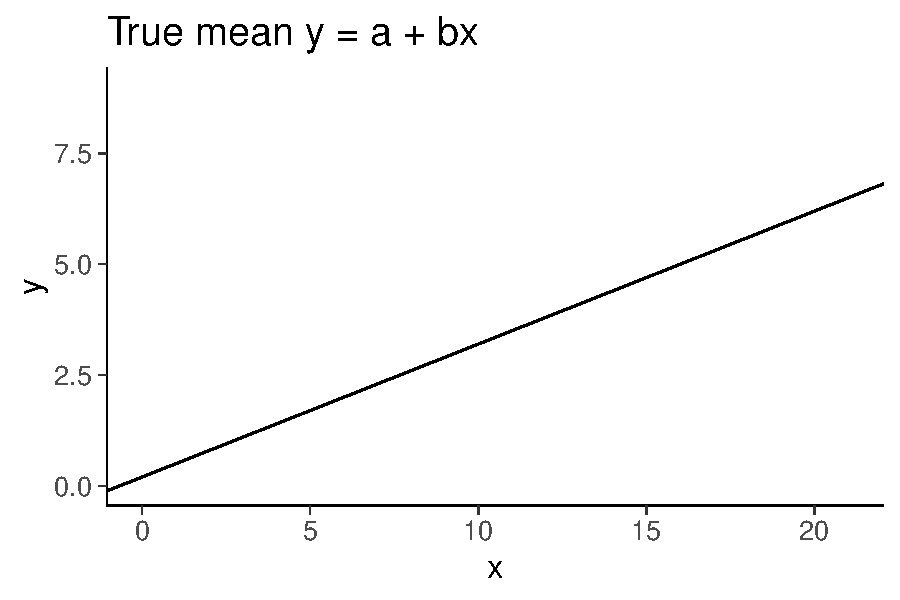
\includegraphics[width=8cm]{figs/fake1.pdf}}
  \only<2>{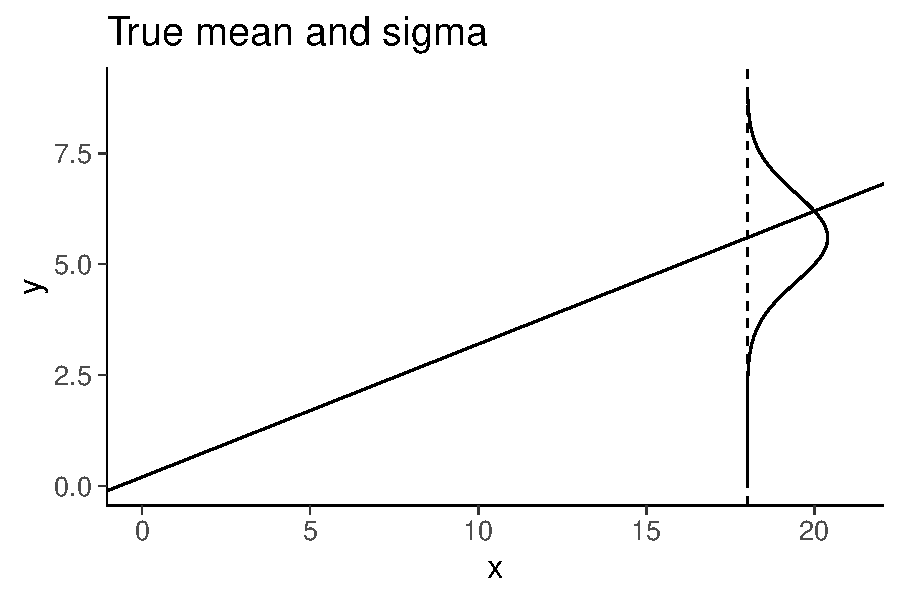
\includegraphics[width=8cm]{figs/fake2.pdf}}
  \only<3>{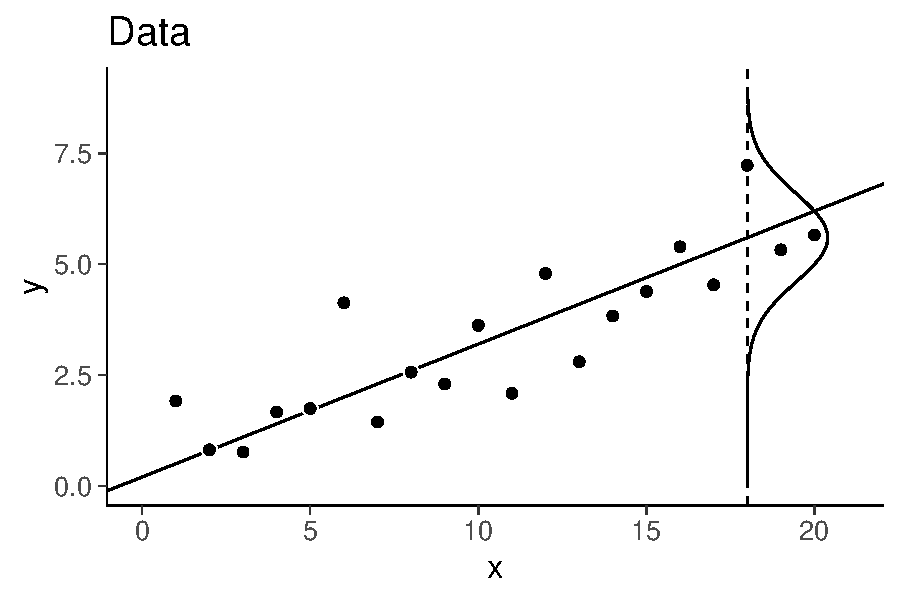
\includegraphics[width=8cm]{figs/fake3.pdf}}
  \only<4>{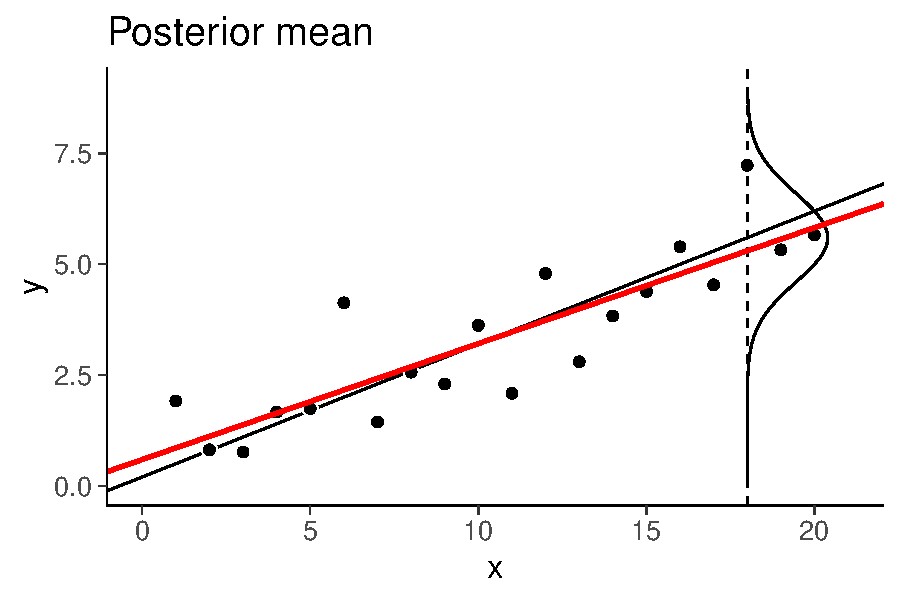
\includegraphics[width=8cm]{figs/fake4.pdf}}
  \only<5>{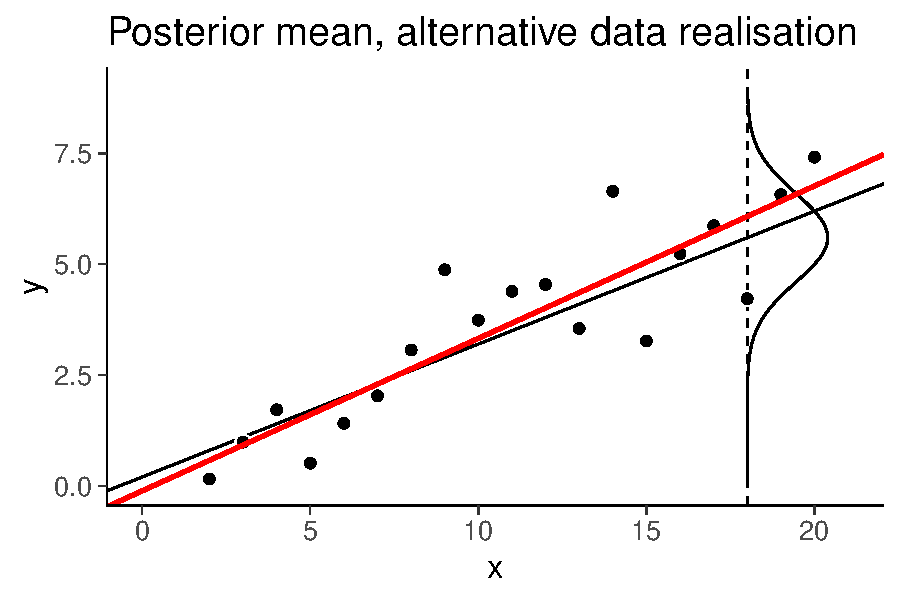
\includegraphics[width=8cm]{figs/fake4b.pdf}}
  \only<6>{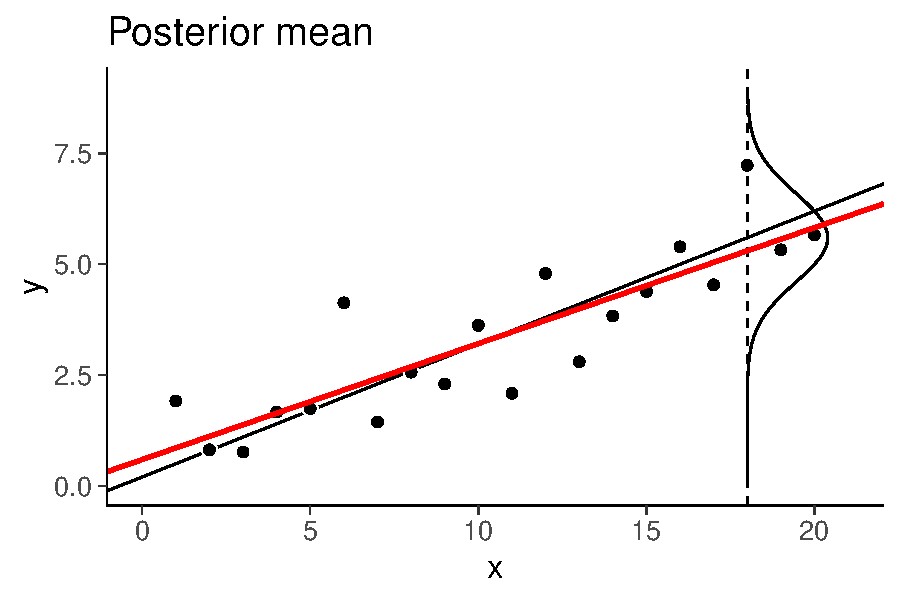
\includegraphics[width=8cm]{figs/fake4.pdf}}
  \only<7>{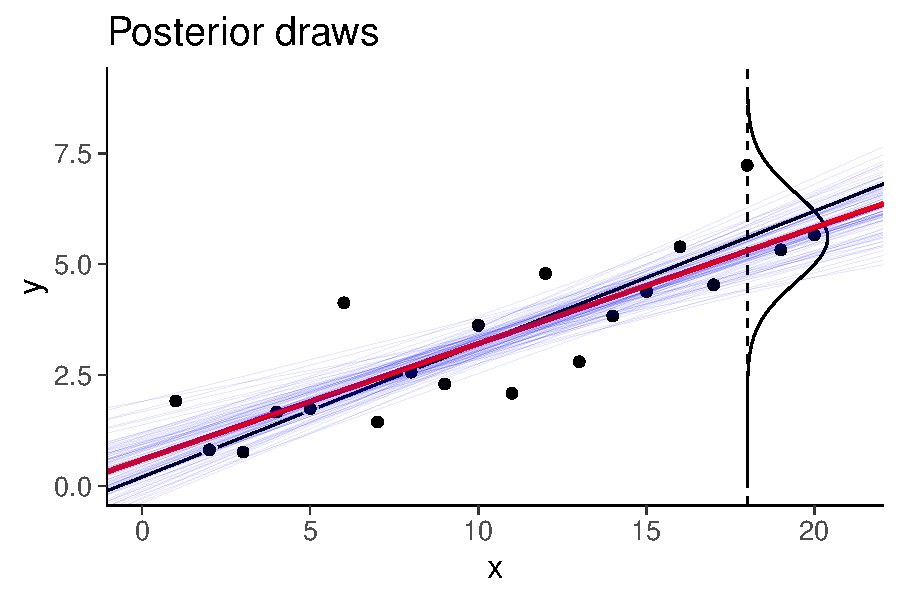
\includegraphics[width=8cm]{figs/fake4s.pdf}}
  \only<8-9>{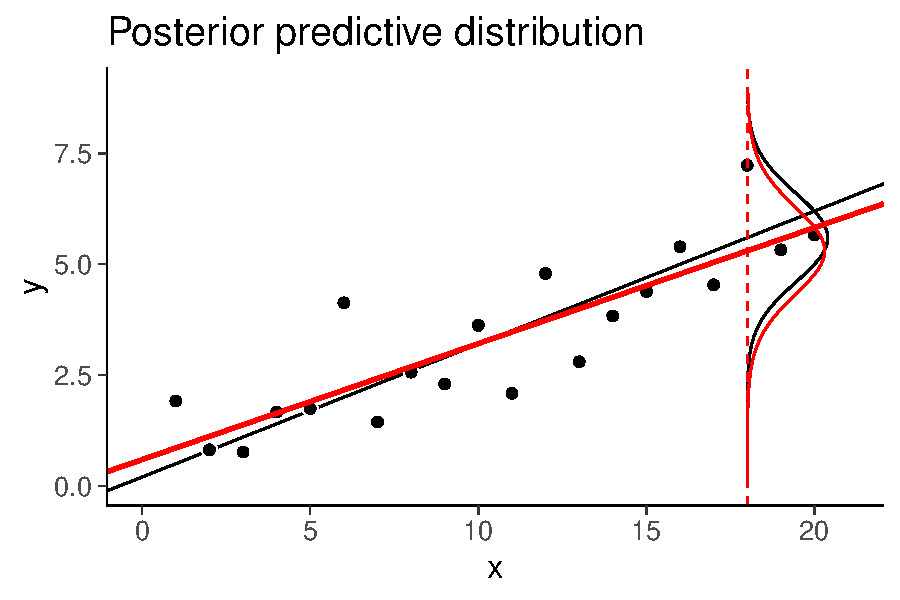
\includegraphics[width=8cm]{figs/fake5.pdf}}
  \only<10>{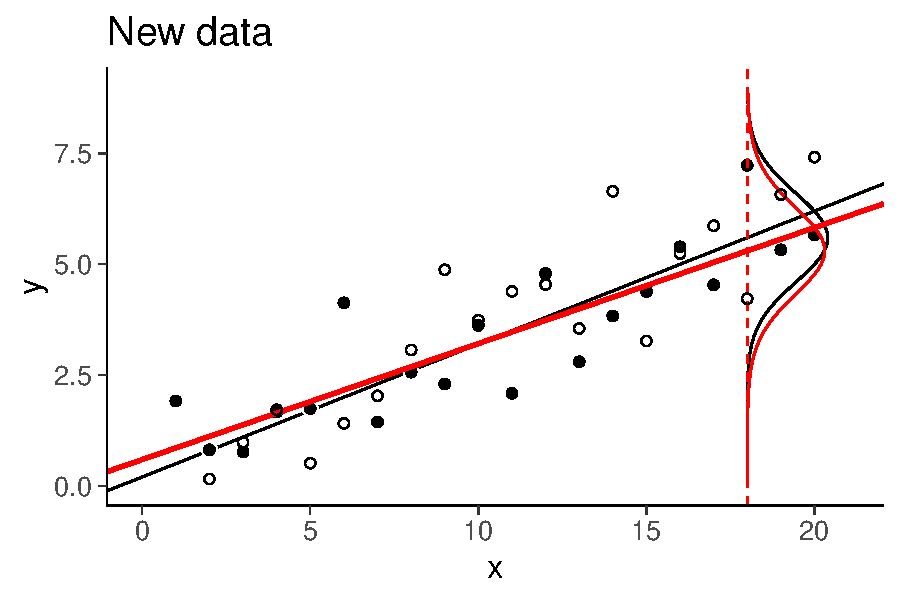
\includegraphics[width=8cm]{figs/fake5n.pdf}}
  \only<11>{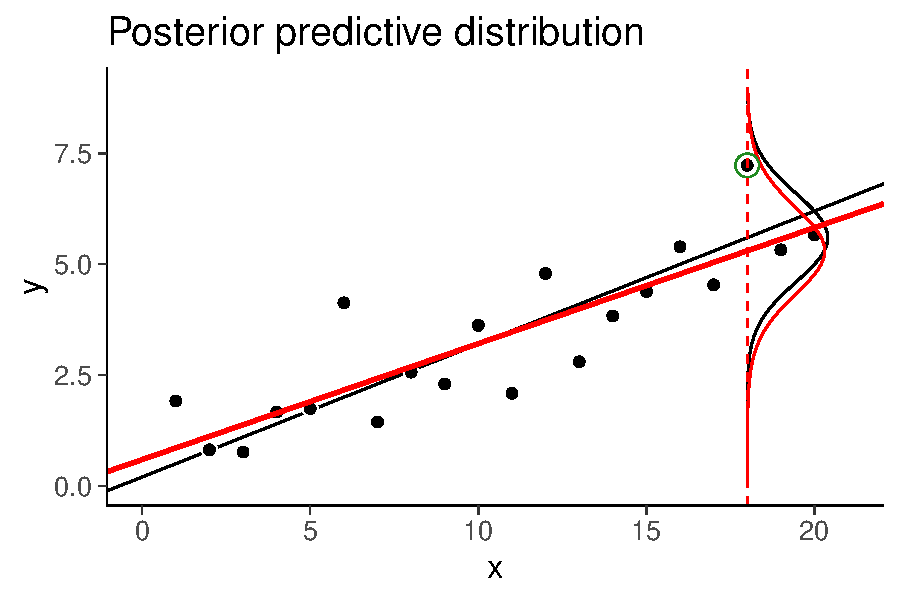
\includegraphics[width=8cm]{figs/fake6.pdf}}
  \only<12>{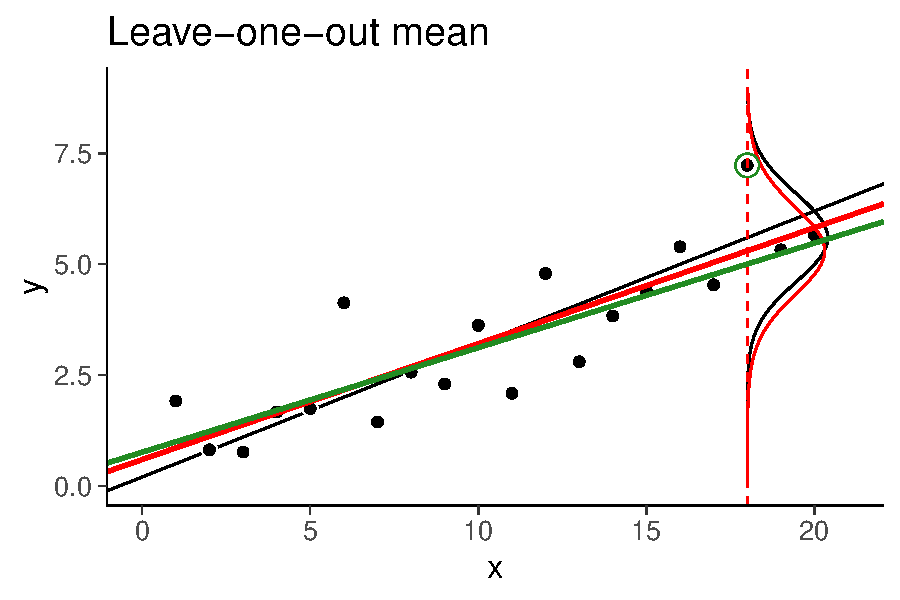
\includegraphics[width=8cm]{figs/fake7.pdf}}
  \\
  \onslide<9>{\color{red} $p(\tilde{y}|\tilde{x}=18,x,y)=\int p(\tilde{y}|\tilde{x}=18,\theta)p(\theta|x,y)d\theta$\\ \vspace{0.5\baselineskip}}
\end{frame}

\begin{frame}{}

  {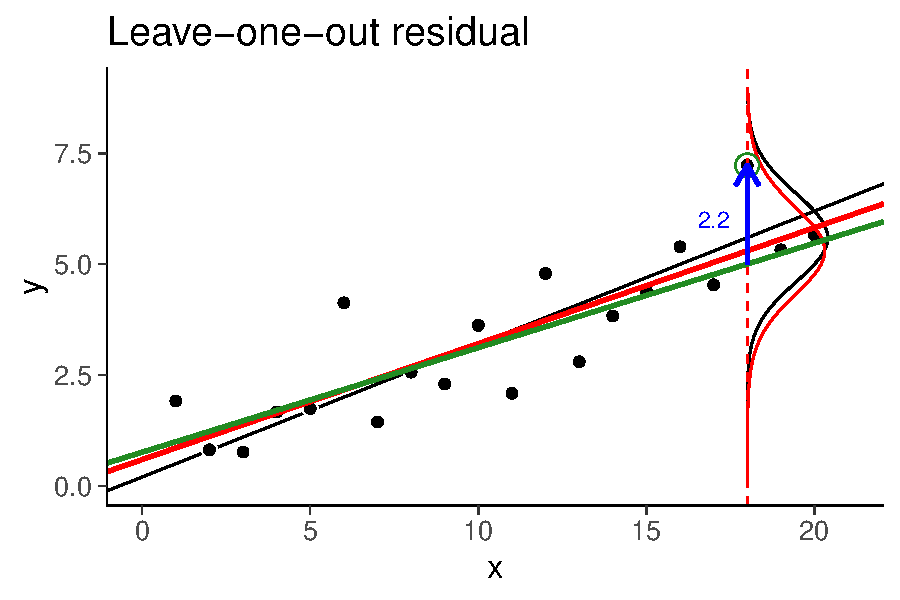
\includegraphics[width=8cm]{figs/fake7r.pdf}}
  \\
  \onslide<2->{{\color{blue} $y_{18} - E[p(\tilde{y}|\tilde{x}=18,x_{-18},y_{-18})]$}\\ \vspace{0.5\baselineskip}}
  \onslide<3->{Can be use to compute, e.g., RMSE, $R^2$, 90\% error}
%  \onslide<4>{\\~\\ \small See LOO-$R^2$ at \url{avehtari.github.io/bayes_R2/bayes_R2.html}}
\end{frame}

\begin{frame}{}

  {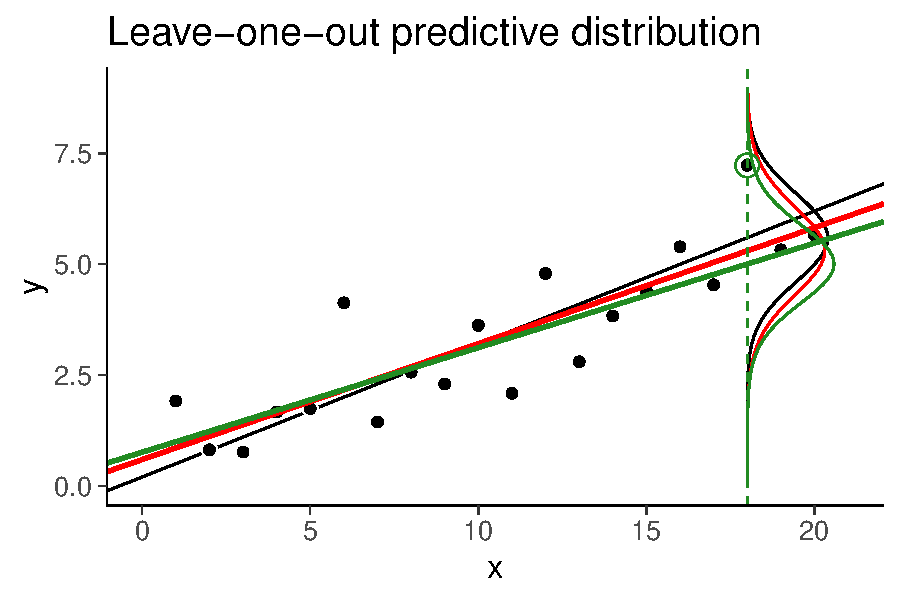
\includegraphics[width=8cm]{figs/fake8.pdf}}
  \\
  \onslide<2>{\color{uulgr} $p(\tilde{y}|\tilde{x}=18,x_{-18},y_{-18})=\int p(\tilde{y}|\tilde{x}=18,\theta)p(\theta|x_{-18},y_{-18})d\theta$}

\end{frame}

\begin{frame}{}

  \only<1-2>{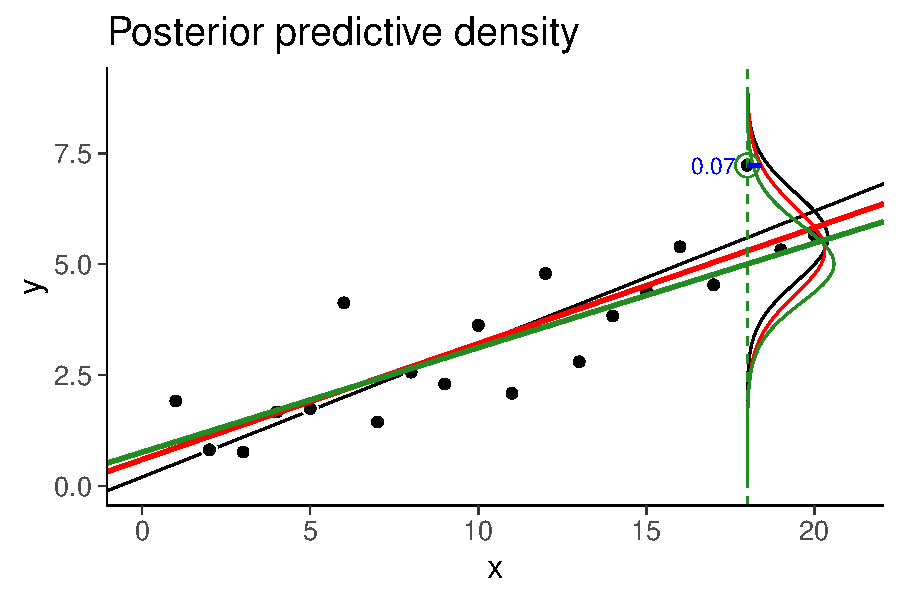
\includegraphics[width=8cm]{figs/fake8pd.pdf}}
  \only<3>{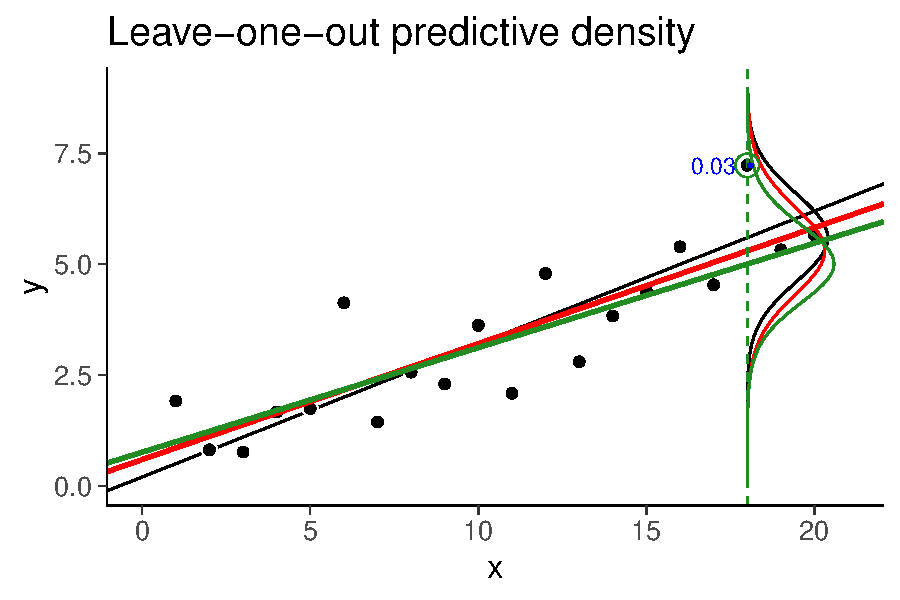
\includegraphics[width=8cm]{figs/fake8loopd.pdf}}
  \\
  \onslide<2->{\color{red} $p(\tilde{y}=y_{18}|\tilde{x}=18,x,y) \approx 0.07$\\ \vspace{0.5\baselineskip}}
  \onslide<3>{\color{uulgr} $p(\tilde{y}=y_{18}|\tilde{x}=18,x_{-18},y_{-18}) \approx 0.03$}

\end{frame}

\begin{frame}{}

  \only<1>{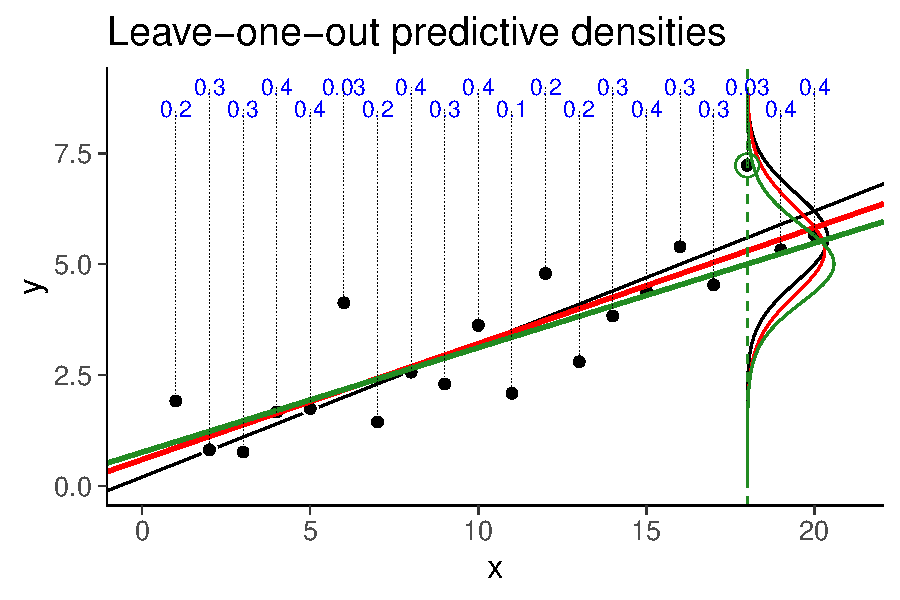
\includegraphics[width=8cm]{figs/fake8loopds.pdf}}
  \only<2->{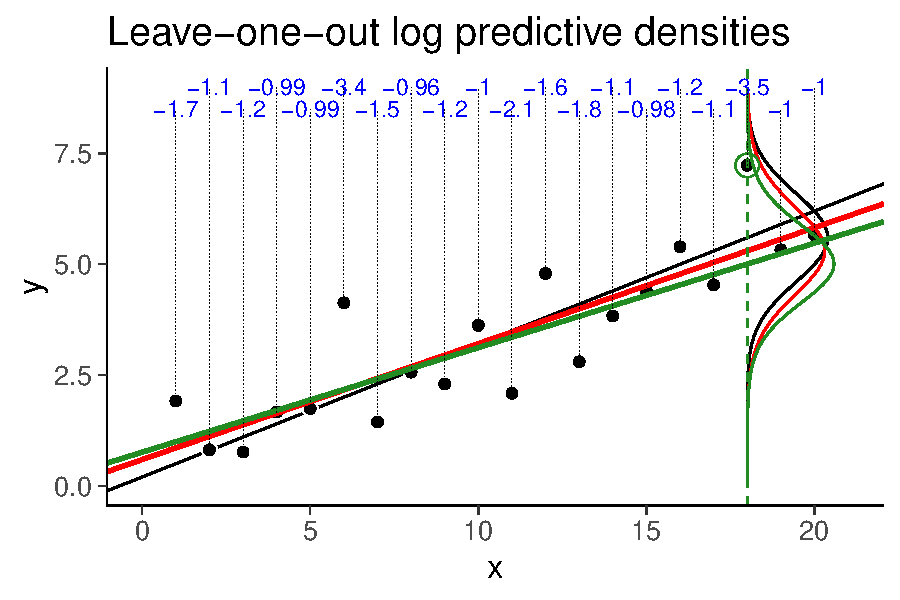
\includegraphics[width=8cm]{figs/fake8loolpds.pdf}}
  \\ \vspace{-0.5\baselineskip}
  \only<1>{\color{blue} $p(y_i|x_i,x_{-i},y_{-i}), \quad i=1,\ldots,20$}
  \only<2>{\color{blue} $\log p(y_i|x_i,x_{-i},y_{-i}), \quad i=1,\ldots,20$}
  \only<3>{\color{blue} $\sum_{i=1}^{20} \log p(y_i|x_i,x_{-i},y_{-i}) \approx -29.5$}
  \only<4->{\color{blue} $\mbox{elpd\_loo} = \sum_{i=1}^{20} \log p(y_i|x_i,x_{-i},y_{-i}) \approx -29.5$\\ \vspace{0.2\baselineskip}}
  \only<5> {\color{blue} unbiased estimate of log posterior pred. density for new data}
  \only<6-7>{\color{red} $\mbox{lpd} = \sum_{i=1}^{20} \log p(y_i|x_i,x,y) \approx -26.8$\\ \vspace{0.2\baselineskip}}
  \only<7>{\color{blue} $\mbox{p\_loo} = \mbox{lpd}-\mbox{elpd\_loo} \approx 2.7$}
  \only<8-> {\color{blue} $\mbox{SE} = \mbox{sd}(\log p(y_i|x_i,x_{-i},y_{-i}))\cdot \sqrt{20} \approx 3.3$}
% TOMOVE:  \only<9>{\\~\\~\\ \color{black} \footnotesize see \href{http://link.springer.com/article/10.1007/s11222-016-9696-4}{Vehtari, Gelman \& Gabry (2017a)} and \href{http://dx.doi.org/10.1214/12-SS102}{Vehtari \& Ojanen (2012)} for more}

\end{frame}

\begin{frame}[fragile]

\frametitle{Stan and {\tt loo} package}

  {\scriptsize
\begin{lstlisting}
 Computed from 4000 by 20 log-likelihood matrix

         Estimate  SE
elpd_loo    -29.5 3.3
p_loo         2.7 1.0
------
Monte Carlo SE of elpd_loo is 0.1.

Pareto k diagnostic values:
                         Count Pct.    Min. n_eff
(-Inf, 0.5]   (good)     18    90.0%   899
 (0.5, 0.7]   (ok)        2    10.0%   459
   (0.7, 1]   (bad)       0     0.0%   <NA>
   (1, Inf)   (very bad)  0     0.0%   <NA>

All Pareto k estimates are ok (k < 0.7).
See help('pareto-k-diagnostic') for details.
\end{lstlisting}
}

\end{frame}


\subsection{When is LOO applicable}
\frame{\subsectionpage}

\begin{frame}

\frametitle{Pro and cons with LOO-CV}

  \begin{enumerate}
  \item[+] Intuitive
  \item[+] Robust
  \item[+] Good theoretical properties
  \pause
  \item[-] Can be costly (naive LOO-CV mean $n$ posterior computations)
  \end{enumerate}

\end{frame}

\begin{frame}

\frametitle{Sometimes cross-validation is not needed}

\vspace{-0.5\baselineskip}

  \begin{itemize}
  \item Posterior predictive checking can be sufficient\\
    \vspace{0.5\baselineskip}
    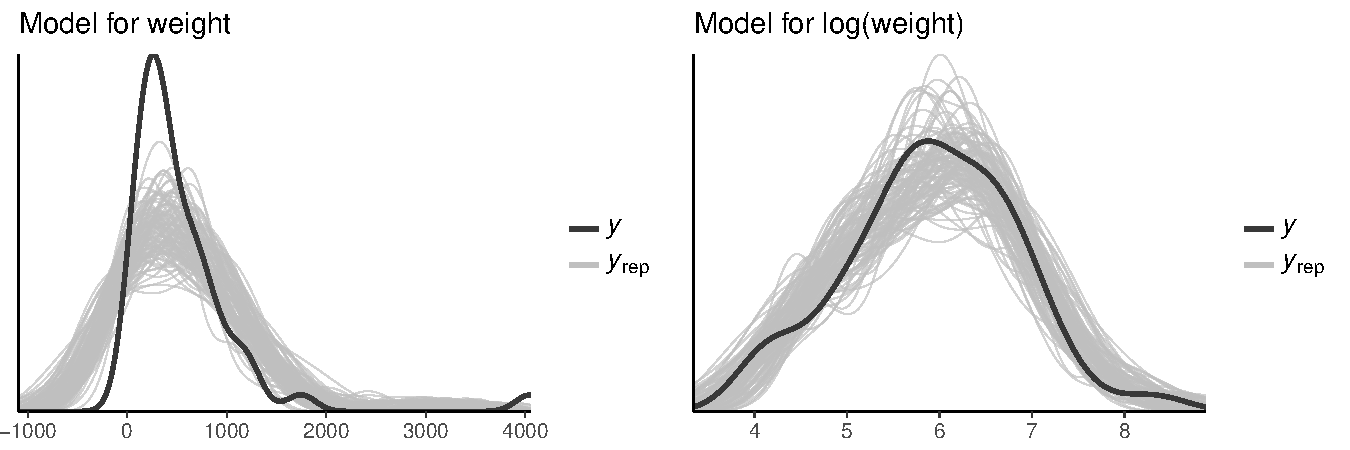
\includegraphics[width=8cm]{figs/mesquite_ppc.pdf}\\
  \vspace{-0.1\baselineskip} {Predicting the yields of mesquite bushes.\\
    \color{gray} \footnotesize
    Gelman, Hill \& Vehtari (2020, Ch. 11)}
  \pause
%  \item For some very simple cases you may assume that true model  is included in the list of models considered % TODO: Add discussion on M-closed etc ($M$-closed)
  \item In nested case, often easier and more accurate to analyse posterior distribution of more complex model directly
  \end{itemize}
%{\footnotesize
%  \begin{enumerate}
%  \item<3-> BDA3, Chapter 6
%  \vspace{-0.6\parskip}
%  \item<3-> Gabry, Simpson, Vehtari, Betancourt, Gelman
%    (2019). Visualization in Bayesian workflow. JRSS A, \url{https://doi.org/10.1111/rssa.12378}
%  \vspace{-0.6\parskip}
%  \item<3-> \url{mc-stan.org/bayesplot/articles/graphical-ppcs.html}
%  \vspace{-0.6\parskip}
%  \item<3-> \url{betanalpha.github.io/assets/case_studies/principled_bayesian_workflow.html}
%   \end{enumerate}}
\end{frame}


%\begin{frame}{}

%\frametitle{Sometimes cross-validation is not needed}

%\begin{enumerate}
%\item<+-> For some very simple cases you may assume that true model
%  is included in the list of models considered ($M$-closed)
%  \begin{enumerate}
%  \item<+-> see predictive model selection in $M$-closed case by
%    San Martini and Spezzaferri (1984)
%  \item<+-> but you should not force your design of experiment or
%    analysis to stay in the simplified world
%  \end{enumerate}
% \item<+-> For fully non-parametric models you may assume that true model
%   is included in the list of models considered ($M$-closed)
%   \begin{enumerate}
%   \item<+-> related to talk by Chris Holmes
%   \item<.-> see
%     \href{http://dx.doi.org/10.1214/12-SS102}{Vehtari \& Ojanen
%       (2012)} for earlier references
% \item<+-> posterior convergence rate can be slow for fully non-parametric models
% \end{enumerate}
%\item<+-> In nested case, often easier and
%  more accurate to analyse posterior distribution of more complex
% model directly %\\
%  {\small \url{avehtari.github.io/modelselection/betablockers.html}}
   % \begin{enumerate}
   %   \item<3-> need to do some model checking anyway
   % \end{enumerate}
%\end{enumerate}

%\end{frame}



\begin{frame}{}

\frametitle{Data generating mechanisms and prediction tasks}

\begin{enumerate}
\item You have to make some assumptions on data generating mechanism $p_\text{true}$
\[
\text{elpd}_M= \int \log p_M({\color{uured}\tilde{y}}|y) p_\text{true}({\color{uured}\tilde{y}}) d{\color{uured}\tilde{y}}\,,
\]
\item Use the knowledge of the prediction task if available
\item Cross-validation can be used to analyse different parts, even if
  there is no clear prediction task
\end{enumerate}

% TODO: Move to recommended reading
% \vspace{6.5\baselineskip}
%{ \small see \href{http://dx.doi.org/10.1214/12-SS102}{Vehtari \& Ojanen (2012)} and \url{andrewgelman.com/2018/08/03/loo-cross-validation-approaches-valid/}}

\end{frame}

% You need to specify the data generating process. this is an assumption
% Approximate how this looks p_true


\begin{frame}{$x$ in $p_\text{true}$}

  \only<1>{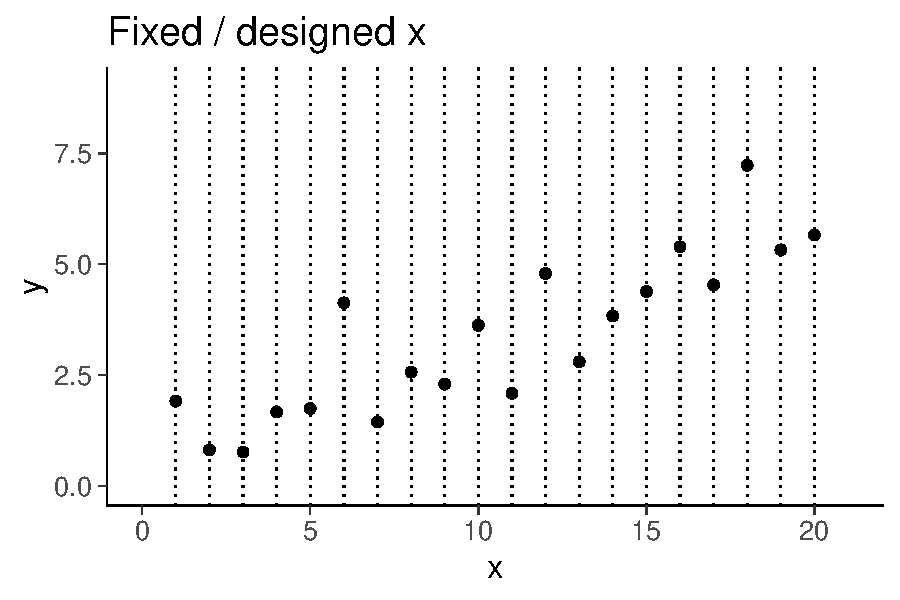
\includegraphics[width=8cm]{figs/fakedfixed.pdf}}
  \only<2->{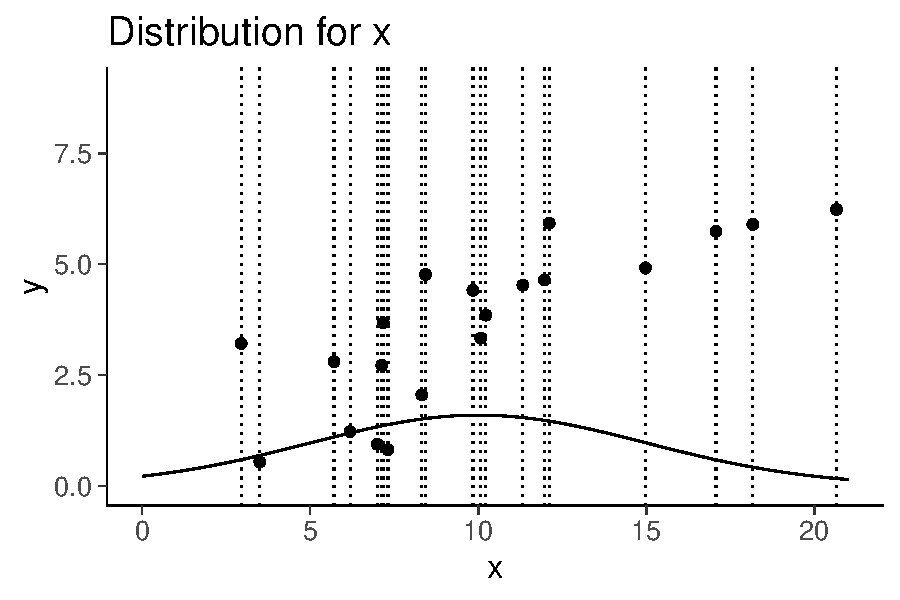
\includegraphics[width=8cm]{figs/fakedrandom.pdf}}
  \\ \vspace{-0.5\baselineskip}
  \only<1>{LOO is ok for fixed / designed $x$: $p_\text{true}(y|x)$}% SE is uncertainty about $y|x$.\\ \vspace{0.2\baselineskip}}
  \only<2->{LOO is ok for random $x$. $p_\text{true}(y,x)$ }%SE is uncertainty about $y|x$ and $x$.\\ \vspace{0.2\baselineskip}}
  %\onslide<3>{Covariate shift can be handled with importance weighting or modelling}
  % TODO: Move to reading
%  \onslide<1->{\\ \small see \href{http://dx.doi.org/10.1214/12-SS102}{Vehtari \& Ojanen (2012)} and \url{andrewgelman.com/2018/08/03/loo-cross-validation-approaches-valid/}}

\end{frame}



\begin{frame}{$p_\text{true}$ extrapolation}

  \only<1>{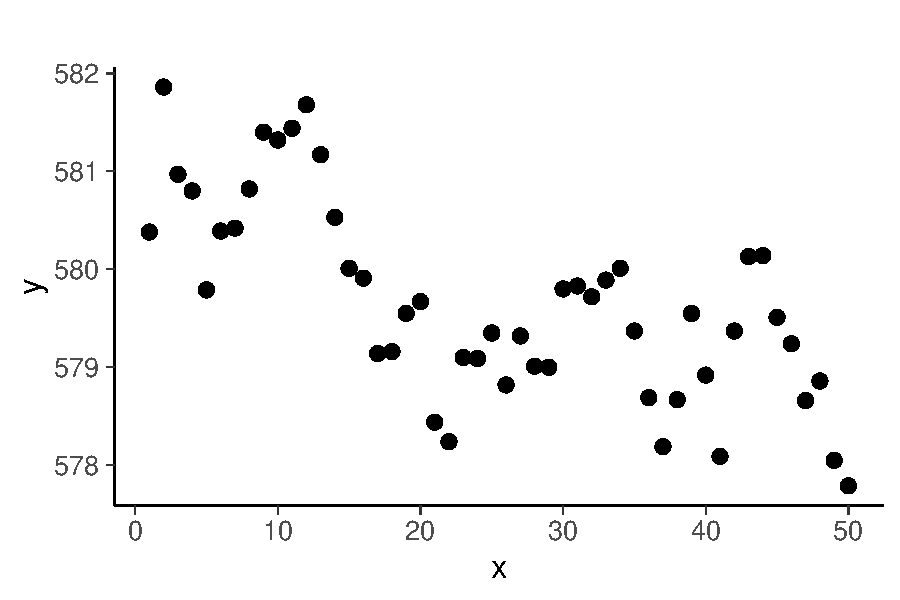
\includegraphics[width=8cm]{figs/lake1data.pdf}}
  \only<2>{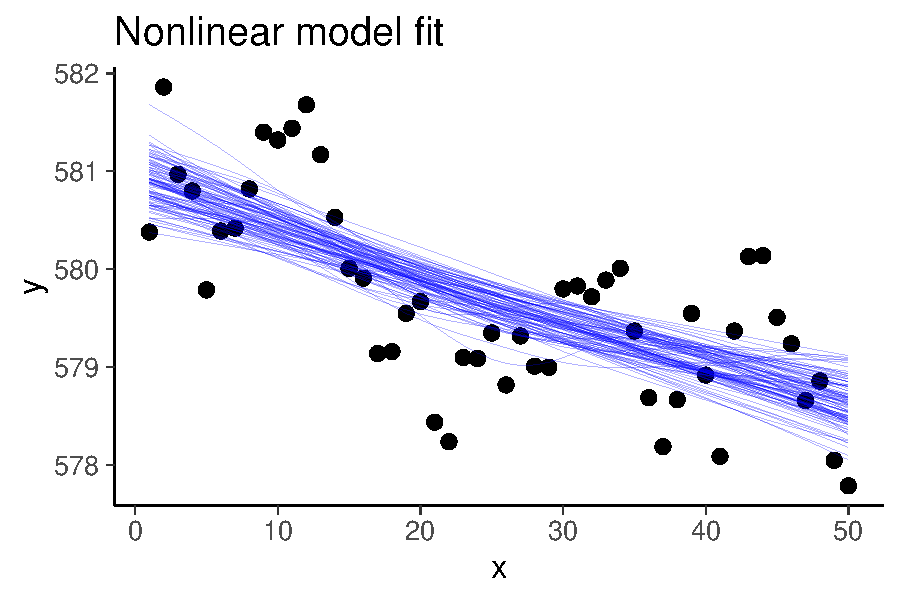
\includegraphics[width=8cm]{figs/lake1gp.pdf}}
  \only<3->{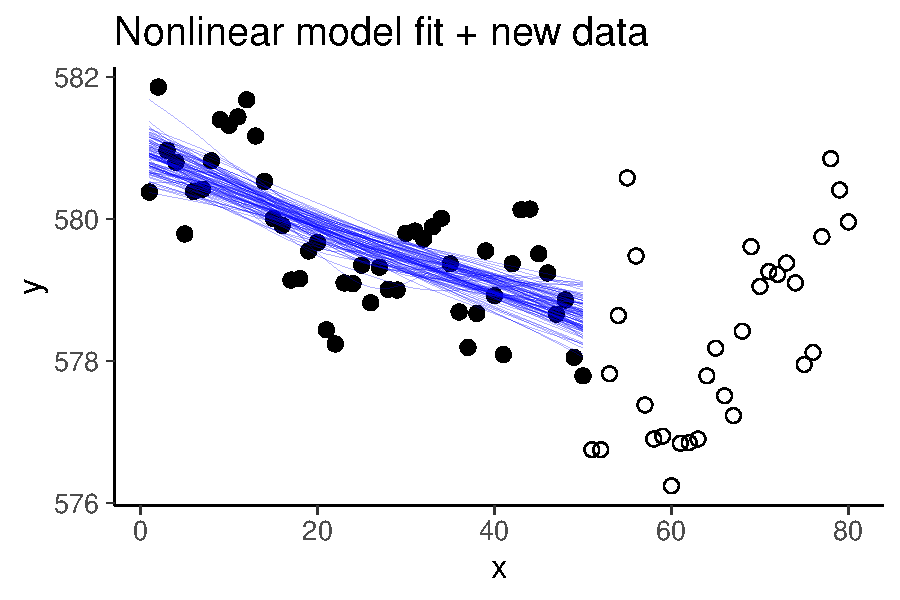
\includegraphics[width=8cm]{figs/lake1gpptest.pdf}}
  \\
  \only<3>{Extrapolation is more difficult}

\end{frame}

\begin{frame}{LOO for time series data}

  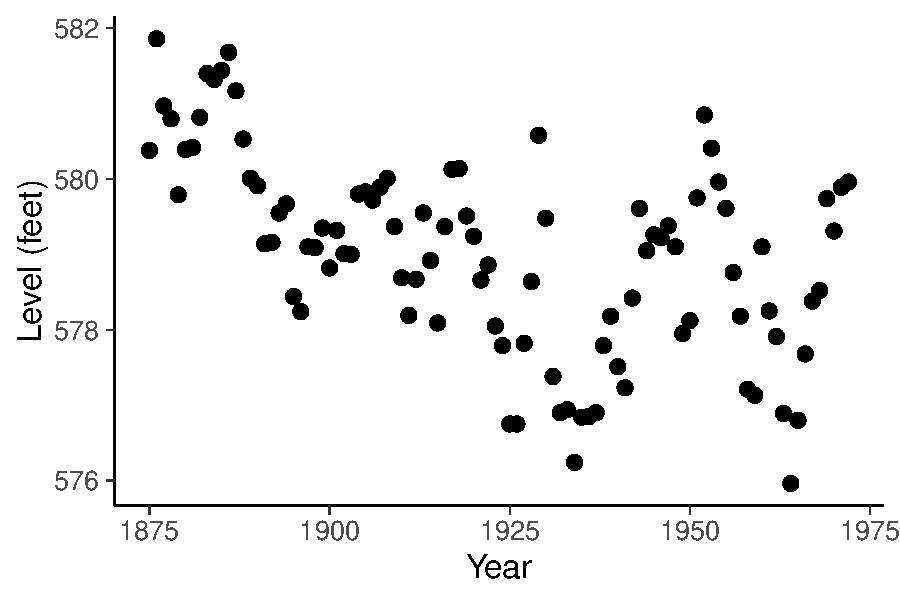
\includegraphics[width=8cm]{figs/lake2data.pdf}

  \centering
  $p_\text{true}$ for time series?

\end{frame}

\begin{frame}{LOO for time series}

  \only<1>{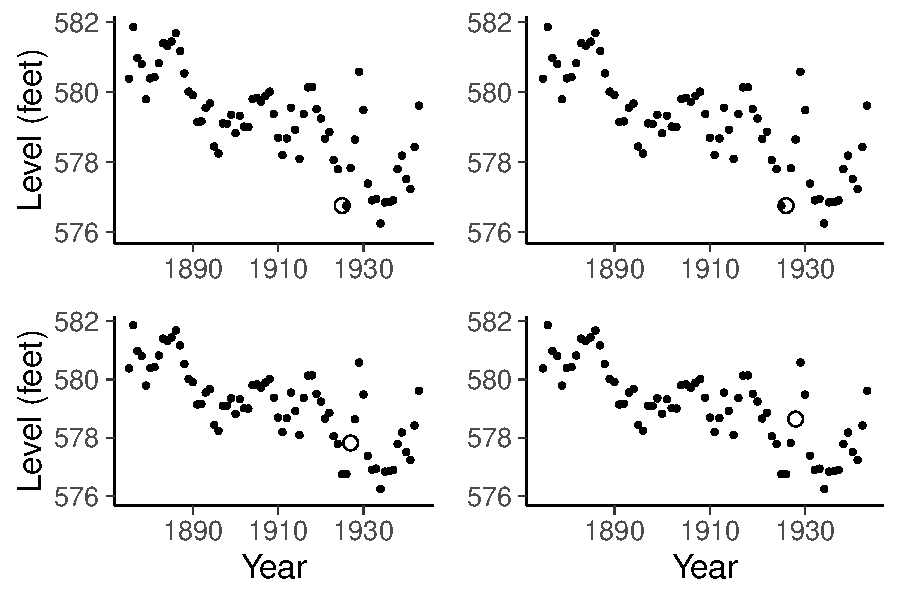
\includegraphics[width=8cm]{figs/lake3loo.pdf}}
  \only<2>{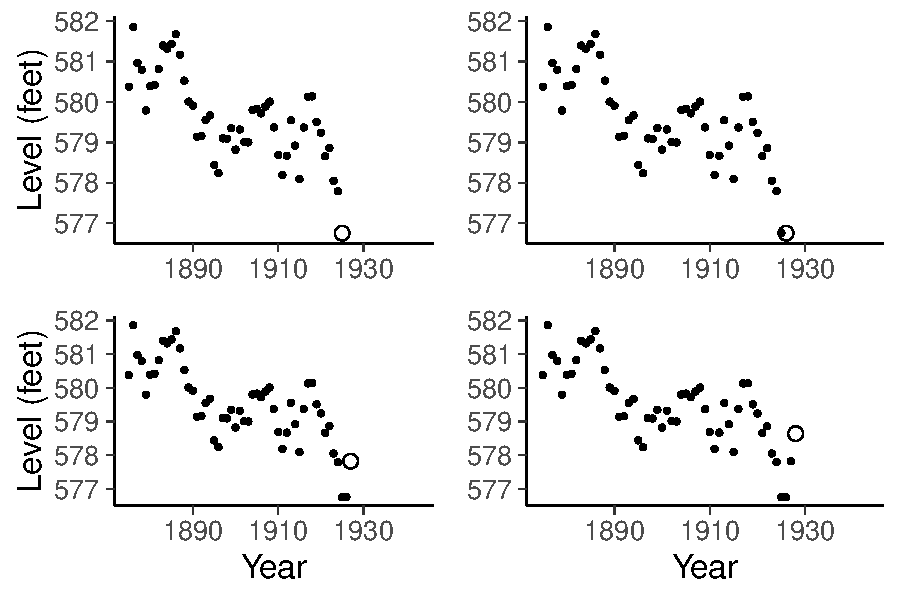
\includegraphics[width=8cm]{figs/lake3stepahead.pdf}}
  \only<3>{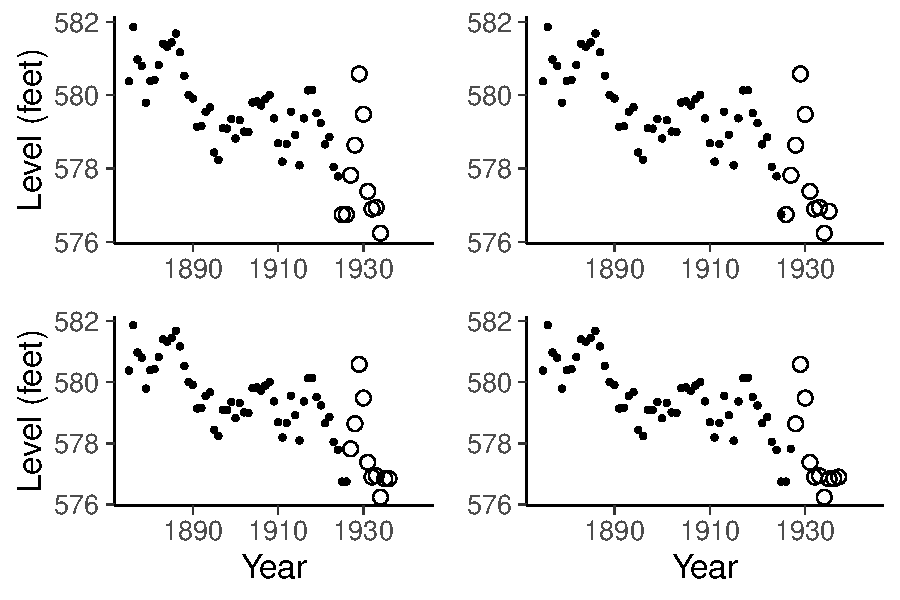
\includegraphics[width=8cm]{figs/lake3tenstepahead.pdf}}
  \only<4>{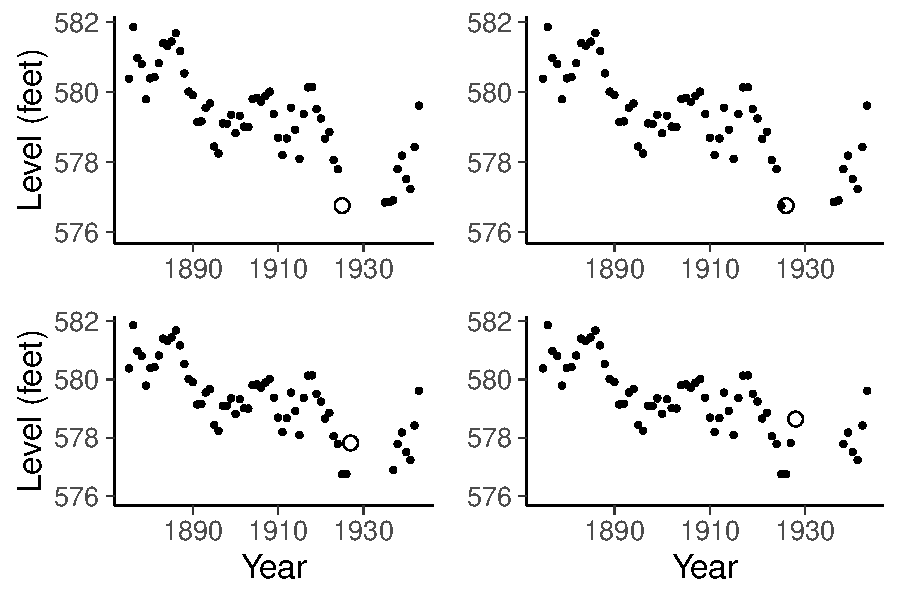
\includegraphics[width=8cm]{figs/lake3stepaheadblock.pdf}}
  \\
  \only<1>{Leave-one-out cross-validation is ok for assessing conditional model}
  \only<2>{Leave-future-out cross-validation is better for predicting future}
  \only<3>{$m$-step-ahead cross-validation is better for predicting further future}
  \only<4>{$m$-step-ahead leave-a-block-out cross-validation}

\end{frame}

\begin{frame}{LOO for hiearchical data}

  \only<1>{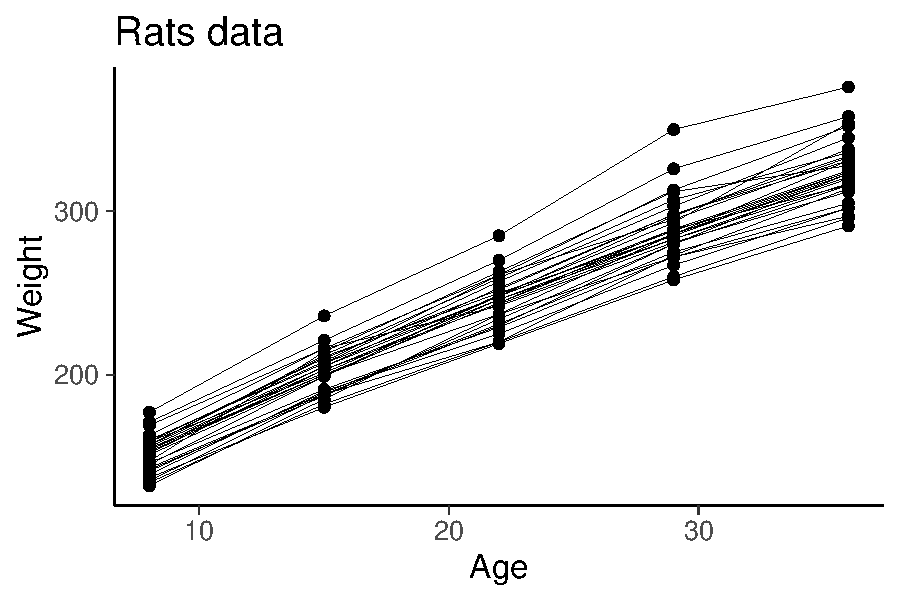
\includegraphics[width=8cm]{figs/rats1data.pdf}}
  \only<2>{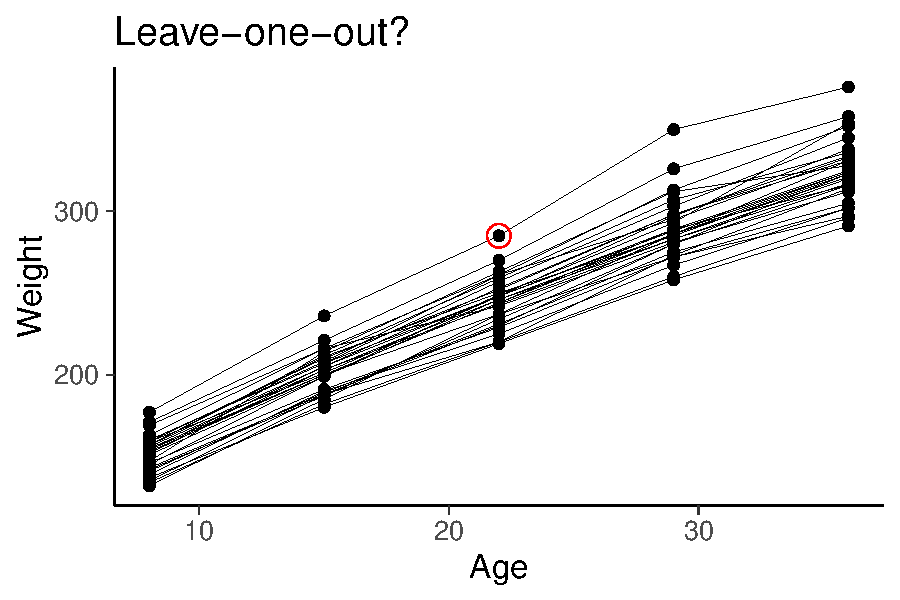
\includegraphics[width=8cm]{figs/rats1loo.pdf}}
  \only<3>{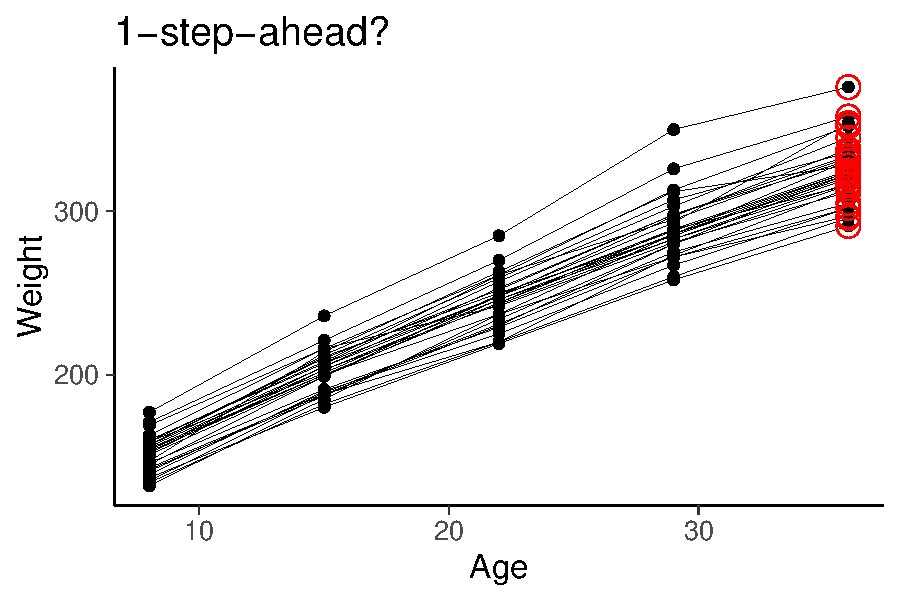
\includegraphics[width=8cm]{figs/rats1step.pdf}}
  \only<4>{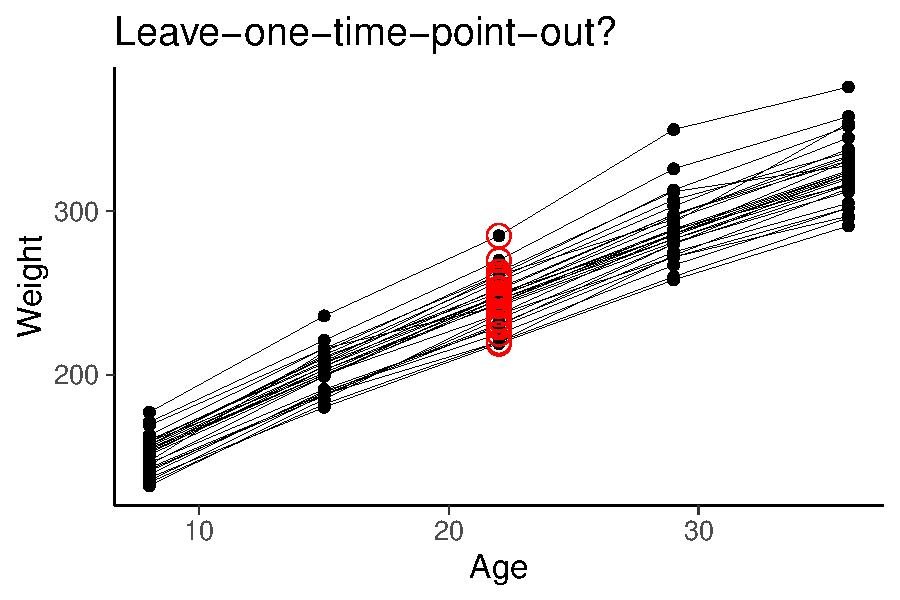
\includegraphics[width=8cm]{figs/rats1onetime.pdf}}
  \only<5>{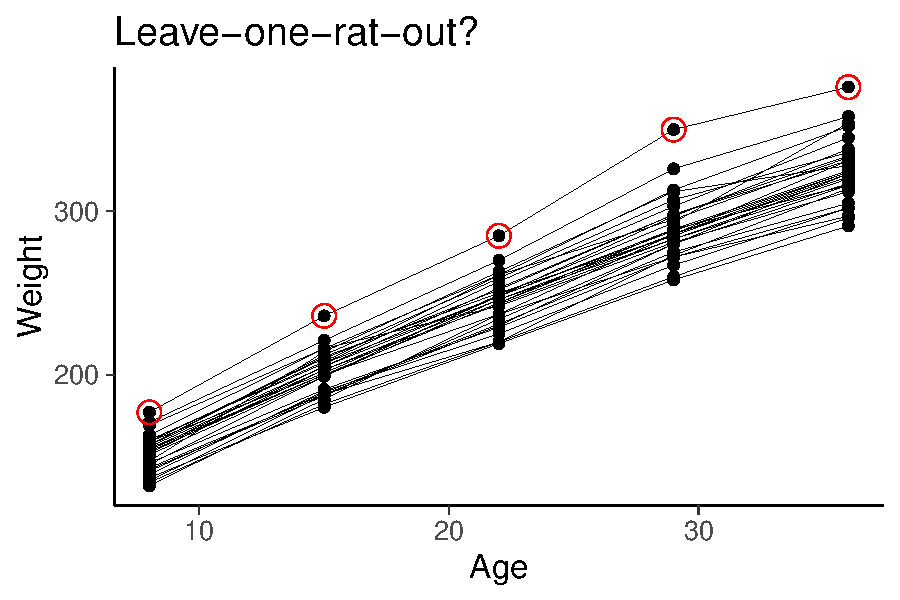
\includegraphics[width=8cm]{figs/rats1onerat.pdf}}
  \only<6>{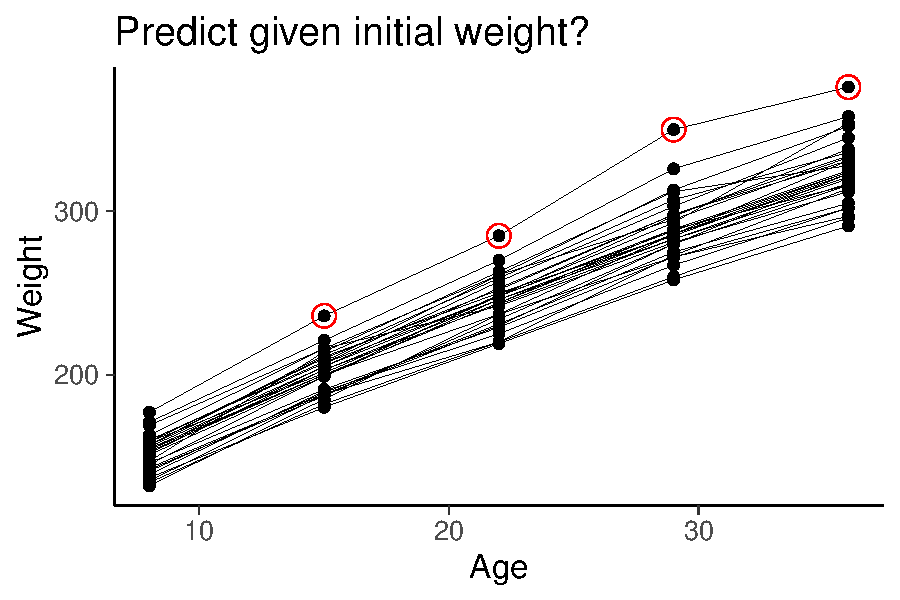
\includegraphics[width=8cm]{figs/rats1init.pdf}}
  \\
  \only<1>{Can LOO or other cross-validation be used with hierarchical data?}
  \only<2->{Yes!}

\end{frame}


\begin{frame}{}

\frametitle{Fast cross-validation}

\begin{enumerate}
\item Pareto smoothed importance sampling LOO (PSIS-LOO)
\pause
\item K-fold cross-validation
\end{enumerate}

\vspace{12\baselineskip}

% TODO: Move
% {\small see \href{http://link.springer.com/article/10.1007/s11222-016-9696-4}{Vehtari, Gelman \& Gabry (2017a)} and \url{mc-stan.org/loo/}}

\end{frame}

\subsection{PSIS LOO-CV}
\frame{\subsectionpage}

\begin{frame}

\frametitle{Recap: Importance sampling}

  %\begin{itemize}
  %   \vspace{-.5\baselineskip}
   %\item[-] Proposal does not need to have a higher value everywhere
   %\end{itemize}
   \begin{center}
     \vspace{-1\baselineskip}
     \only<1-2>{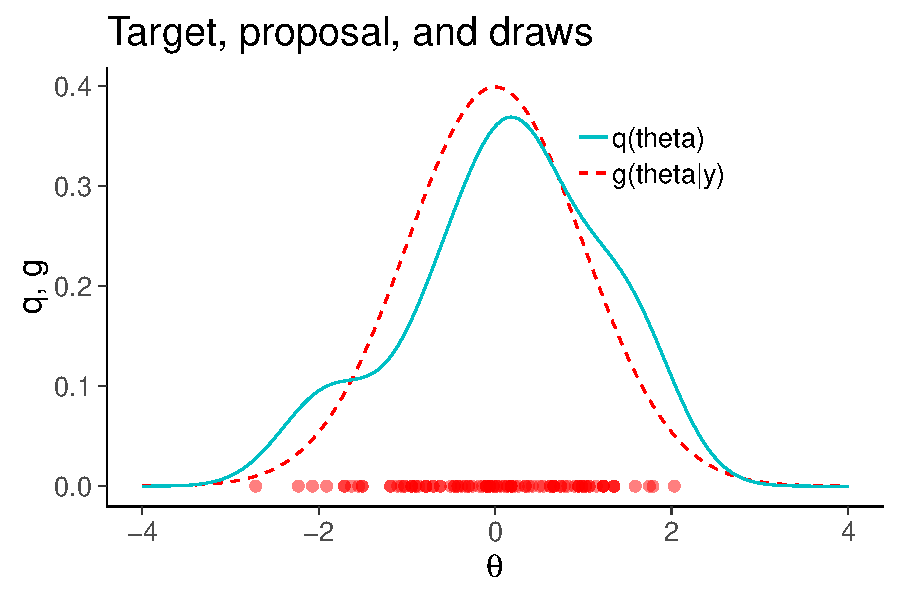
\includegraphics[width=9cm]{figs/importancesamp1.pdf}}
     \only<3>{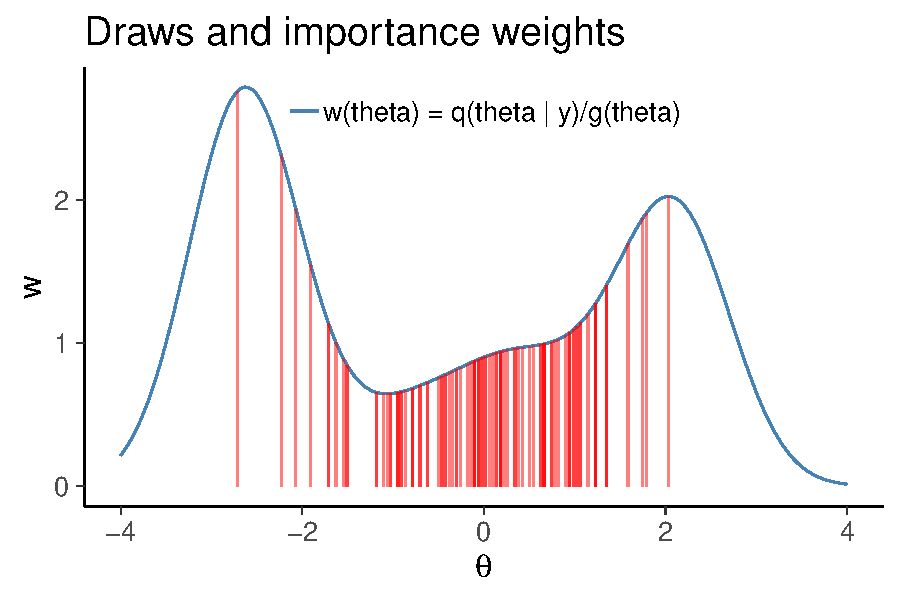
\includegraphics[width=9cm]{figs/importancesamp2.pdf}}
     \vspace{-1\baselineskip}
     \only<2->{
   \begin{eqnarray*}
      \E[f(\theta)] \approx \frac{\sum_s w_s f(\theta^{(s)})}{\sum_s
      w_s}, \qquad \text{where} \quad
      w_s =  \frac{q(\theta^{(s)})}{g(\theta^{(s)})} \qquad
   \end{eqnarray*}
   }
   \end{center}

\end{frame}



\begin{frame}
  \frametitle{Importance sampling for LOO-CV}

   \begin{itemize}
   \item Let $f = p(\tilde{y}_i|y_{-i})$, $g = p(\theta|y)$, and $q = p(\theta|y_{-i})$
   \pause
   \item Having samples $\theta^s$ from $p(\theta^s|y)$
     \begin{align*}
       p(\tilde{y}_i|y_{-i})\approx\frac{\sum_{s=1}^S p(\tilde{y}_i|\theta^s) w_i^s}{\sum_{s=1}^S w_i^s},
     \end{align*}
     where $w_i^s$ are importance weights and
     \begin{align*}
       w_i^s=\frac{p(\theta^s|y_{-i})}{p(\theta^s|y)}.
     \end{align*}
   \end{itemize}

 \end{frame}

\begin{frame}
  \frametitle{Importance sampling for LOO-CV}

   \begin{itemize}
   \item We get a nice solution
     \begin{align*}
       w_i^s=\frac{p(\theta^s|y_{-i})}{p(\theta^s|y)} = \frac{\frac{p(\theta^s) \prod_{j \neq i} p(y_j | \theta^s)}{p(y_{-i})}}{\frac{p(\theta^s) \prod_j p(y_j | \theta^s)}{p(y)}}\propto\frac{1}{\color{red} p(y_i|\theta^s)}.
     \end{align*}
 \pause
   \item If evaluated with $\tilde{y}_i=y_i$
        \begin{align*}
       p(\tilde{y}_i|y_{-i})\approx\frac{\sum_{s=1}^S p(\tilde{y}_i|\theta^s) w_i^s}{\sum_{s=1}^S w_i^s} = \frac{1}{\sum_{s=1}^S\frac{1}{p(y_i|\theta^s)}},
     \end{align*}
     and
    \begin{align*}
       \log w^{(s)}_i = - \log p(y_i|\theta^{(s)}) %= - \text{log_lik[i]}
    \end{align*}
%    \pause
%    \item What $\theta^{(s)}$ will give large weights?
% TODO: Add normal likelihood with known variance and compute the weights as an example.
   \end{itemize}
 \end{frame}


\begin{frame}{}

  \only<1>{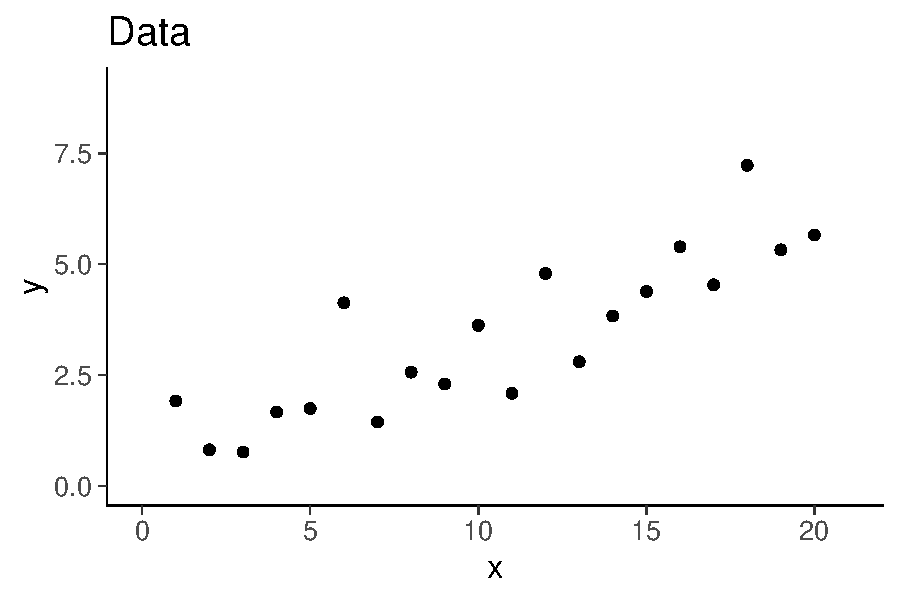
\includegraphics[width=8cm]{figs/fakedata.pdf}}
  \only<2>{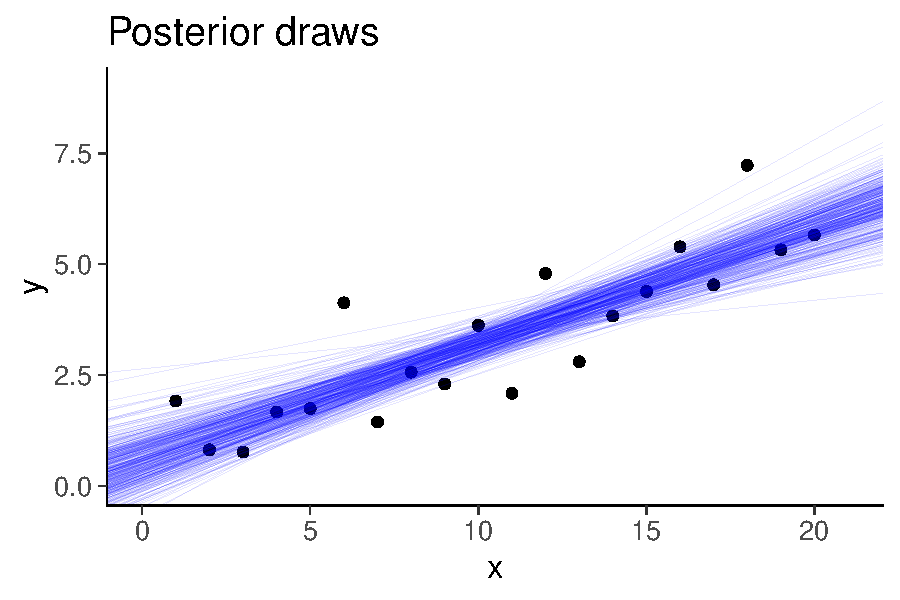
\includegraphics[width=8cm]{figs/fakedraws.pdf}}
  \only<3>{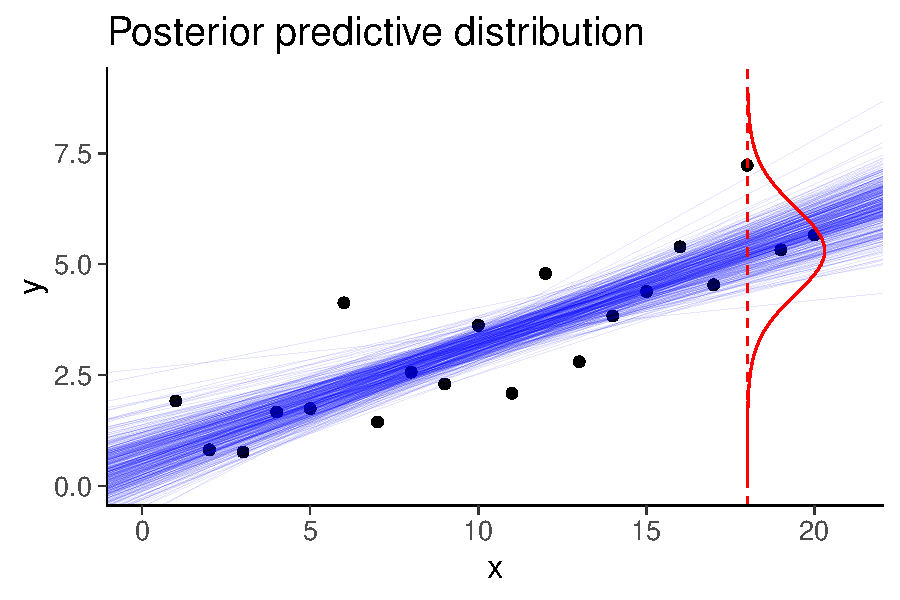
\includegraphics[width=8cm]{figs/fakepostpred.pdf}}
  \only<4>{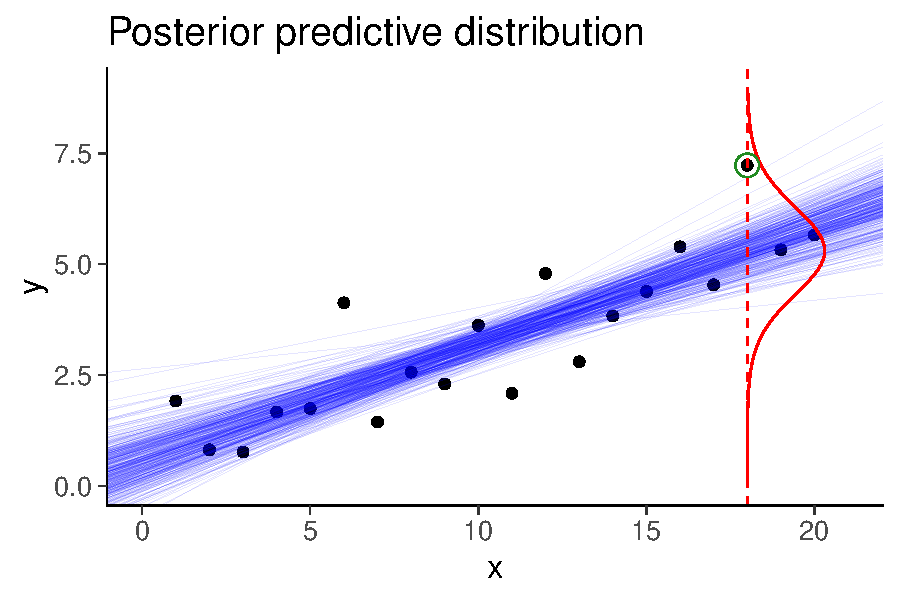
\includegraphics[width=8cm]{figs/fakepostpred18.pdf}}
  \only<5-7>{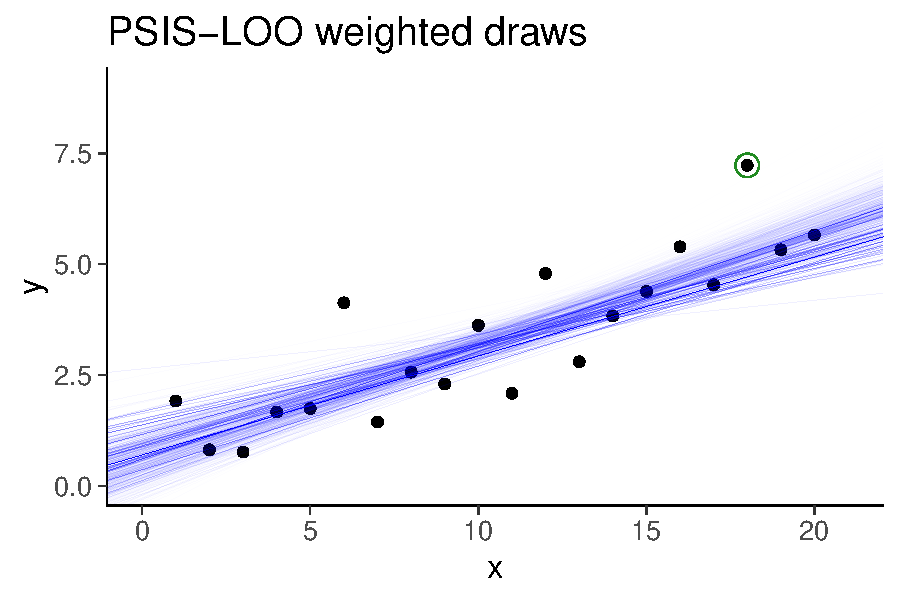
\includegraphics[width=8cm]{figs/fakepsisdraws.pdf}}
  \only<8-10>{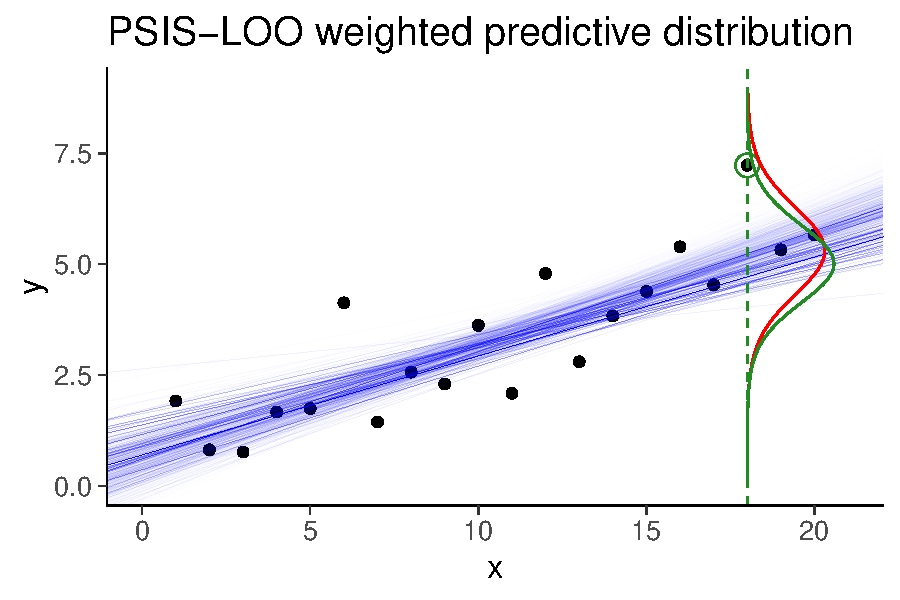
\includegraphics[width=8cm]{figs/fakepsispostpred.pdf}}
  \\
  \only<2>{$\theta^{(s)} \sim p(\theta|x,y)$}
  \only<3-4>{$\theta^{(s)} \sim p(\theta|x,y), \quad p(\tilde{y}|\tilde{x},x,y) \approx \frac{1}{S}\sum_{s=1}^S p(\tilde{y}|\tilde{x},\theta^{(s)})$ }
  \only<5>{$\theta^{(s)} \sim p(\theta|x,y)$\\ \vspace{0.2\baselineskip}$ w_i^{(s)} = p(\theta^{(s)}|x_{-i},y_{-i}) / p(\theta^{(s)}|x,y)$ }
  \only<6-8>{$\theta^{(s)} \sim p(\theta|x,y)$\\ \vspace{0.2\baselineskip} $ w_i^{(s)} = p(\theta^{(s)}|x_{-i},y_{-i}) / p(\theta^{(s)}|x,y) \propto 1/p(y_i|x_i,\theta^{(s)})$\\ \vspace{0.2\baselineskip} }
  \only<7>{$\log(1/p(y_i|x_i,\theta^{(s)})) = -\mbox{log\_lik}[i]$}
  \only<9-10>{$\theta^{(s)} \sim p(\theta|x,y)$\\ \vspace{0.2\baselineskip}
    $ w_i^{(s)} = p(\theta^{(s)}|x_{-i},y_{-i}) / p(\theta^{(s)}|x,y) \propto 1/p(y_i|x_i,\theta^{(s)})$\\ \vspace{0.2\baselineskip}
  $p(y_i|x_i,x_{-i},y_{-i}) \approx \sum_{s=1}^S [w_i^{(s)} p(y_i|x_i,\theta^{(s)})]$}%\only<10>{, where $w \leftarrow \mbox{PSIS}(r)$}

\end{frame}

\begin{frame}

\frametitle{Recap: Pareto smoothed importance sampling}

  \begin{itemize}
  \item Pareto-Smoothed Importance sampling smooth the weights according to a Generalized Pareto($k$) distribution
  \item Pareto-$k$ diagnostic estimate the number of existing moments ($\lfloor 1/k \rfloor$)
  \item<2-> Finite variance and central limit theorem for $k<1/2$
  \item<3-> Finite mean and generalized central limit theorem for $k<1$,
    but pre-asymptotic constant grows impractically large for $k>0.7$
  \item<4-> Hence $k>0.7$ can be used to indicate what observation that can "hold-out" using IS
  \end{itemize}
\end{frame}


\begin{frame}{}

  \only<1>{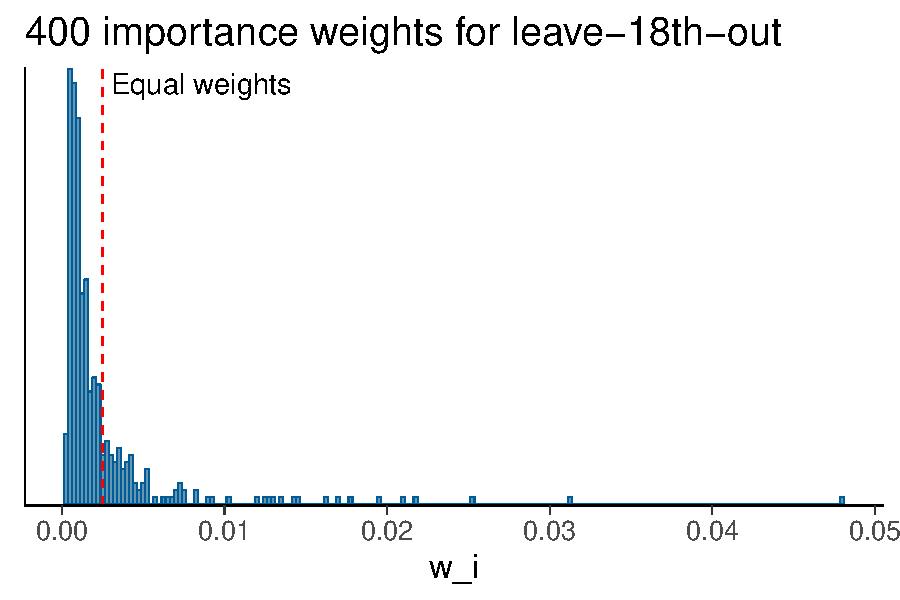
\includegraphics[width=8cm]{figs/fakepsisweights.pdf}}
  \only<2->{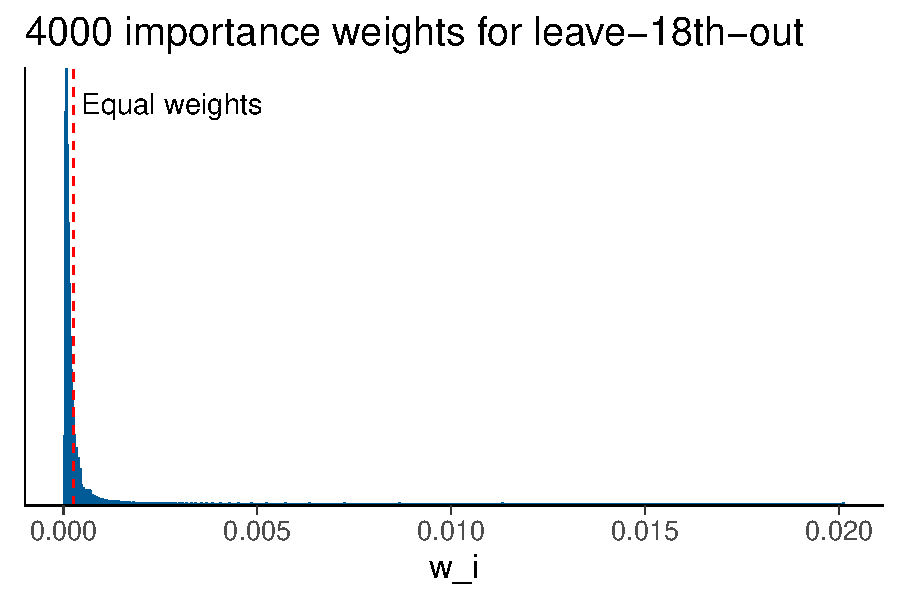
\includegraphics[width=8cm]{figs/fakepsisweights4000.pdf}}
  \\
  \vspace{-\baselineskip}
  \onslide<3->{n\_eff $\approx$ 459\\  \vspace{0.2\baselineskip}}
  \onslide<4>{Pareto $\hat{k}$ $\approx$ 0.52
  \vspace{-\parskip}
Pareto $\hat{k}$ estimates the tail shape which determines the convergence rate of PSIS. Less than 0.7 is ok.}
% TODO: Move to reading  \onslide<3->{\vspace{0.1\baselineskip}\small see \href{http://link.springer.com/article/10.1007/s11222-016-9696-4}{Vehtari, Gelman \& Gabry (2017b)}}
\end{frame}

\begin{frame}[fragile]

  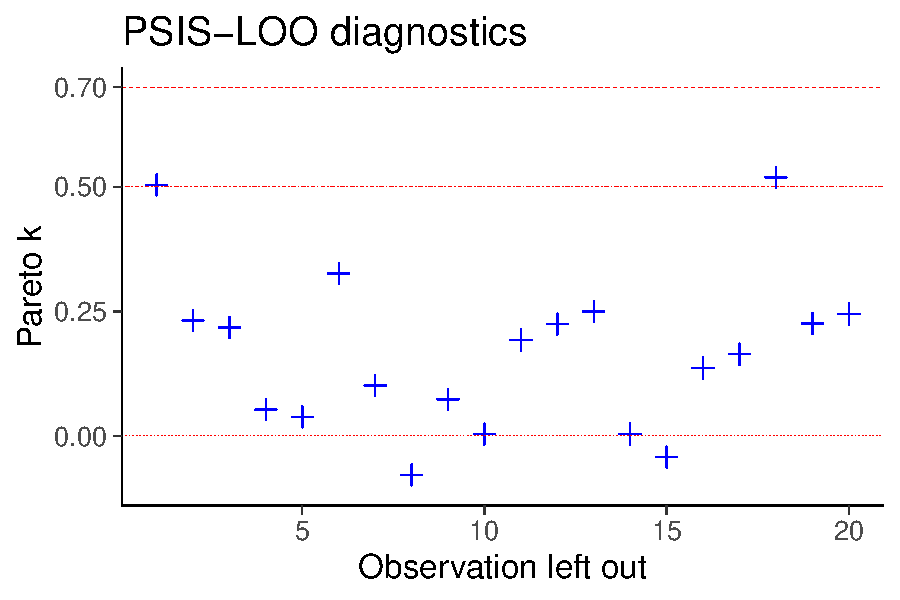
\includegraphics[width=8cm]{figs/fakepks.pdf}

\end{frame}

\begin{frame}[fragile]

  \only<1>{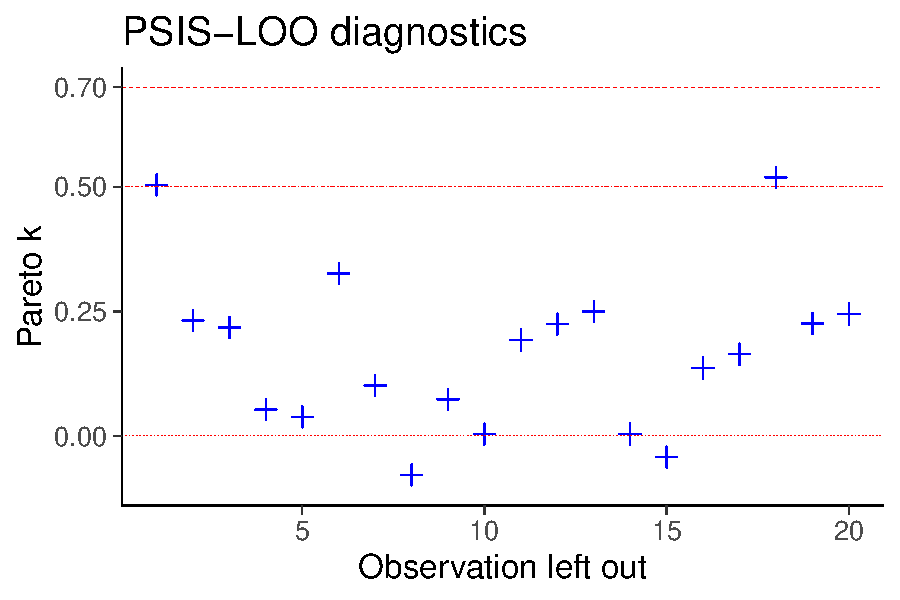
\includegraphics[width=8cm]{figs/fakepks.pdf}}
  \only<2>{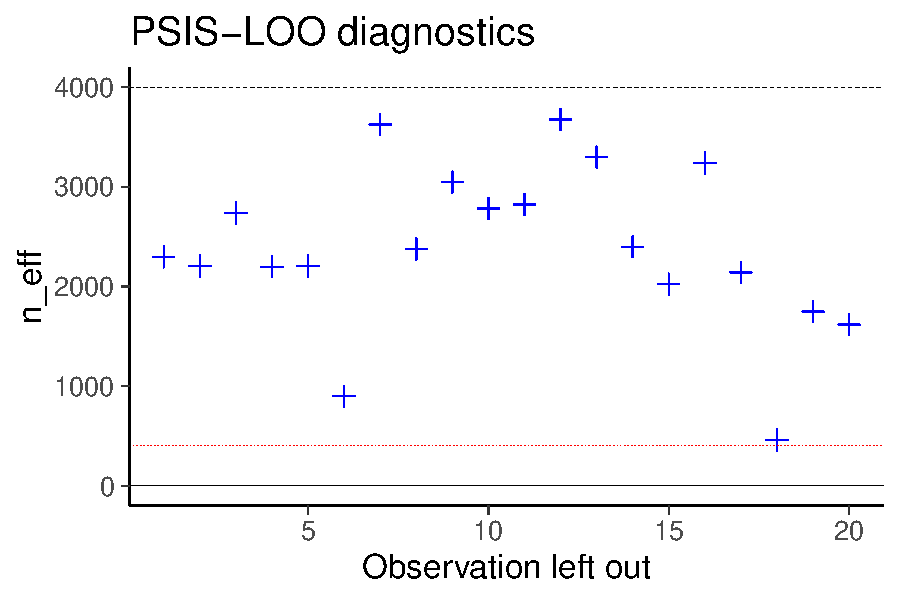
\includegraphics[width=8cm]{figs/fakeneffs.pdf}}
  \\
  {\scriptsize
\begin{lstlisting}
    Pareto k diagnostic values:
                         Count Pct.    Min. n_eff
(-Inf, 0.5]   (good)     18    90.0%   899
 (0.5, 0.7]   (ok)        2    10.0%   459
   (0.7, 1]   (bad)       0     0.0%   <NA>
   (1, Inf)   (very bad)  0     0.0%   <NA>
\end{lstlisting}
}

\end{frame}

\begin{frame}[fragile]
\frametitle{Stan code}

  \vspace{\baselineskip}
  $ \log(w_i^{(s)}) = \log(1/p(y_i|x_i,\theta^{(s)})) = {\color{red}-\mbox{log\_lik}[i]}$
  \vspace{\baselineskip}

  \pause
  {\small
\begin{lstlisting}[language=Stan,escapechar=!]
...
model {
  alpha ~ normal(pmualpha, psalpha);
  beta ~ normal(pmubeta, psbeta);
  y ~ normal(mu, sigma);
}
generated quantities {
  vector[N] log_lik;
  for (i in 1:N)
    !\color{red}\tt log\_lik[i] = normal\_lpdf(y[i] | mu[i], sigma); \color{black}!
}
\end{lstlisting}
  }

\end{frame}

\begin{frame}[fragile]
\frametitle{Stan and {\tt loo} package}

  {\scriptsize
\begin{lstlisting}
 Computed from 4000 by 20 log-likelihood matrix

         Estimate  SE
elpd_loo    -29.5 3.3
p_loo         2.7 1.0
------
Monte Carlo SE of elpd_loo is 0.1.

Pareto k diagnostic values:
                         Count Pct.    Min. n_eff
(-Inf, 0.5]   (good)     18    90.0%   899
 (0.5, 0.7]   (ok)        2    10.0%   459
   (0.7, 1]   (bad)       0     0.0%   <NA>
   (1, Inf)   (very bad)  0     0.0%   <NA>

All Pareto k estimates are ok (k < 0.7).
See help('pareto-k-diagnostic') for details.
\end{lstlisting}
}

\end{frame}

\begin{frame}
\frametitle{PSIS-LOO}

\begin{enumerate}
  \item PSIS-LOO for hierarchical models
  \begin{enumerate}
  \item leave-one-group out is challenging for PSIS-LOO
  %\\ \vspace{0.2\baselineskip}
%    {\small see Merkel, Furr and Rabe-Hesketh
%      (2018) for an approach using quadrature integration}
  \end{enumerate}
  \item<2-> PSIS-LOO for non-factorizable models
  %  \begin{enumerate}
 %   \item {\url{mc-stan.org/loo/articles/loo2-non-factorizable.html}}
%    \end{enumerate}
  \item<3-> PSIS-LOO for time series
  \begin{enumerate}
  \item Approximate leave-future-out cross-validation %\\ \vspace{0.2\baselineskip}
%    {\url{mc-stan.org/loo/articles/loo2-lfo.html}}
  \end{enumerate}
\end{enumerate}

\end{frame}

\begin{frame}{PSIS-LOO for time series}

  \only<1>{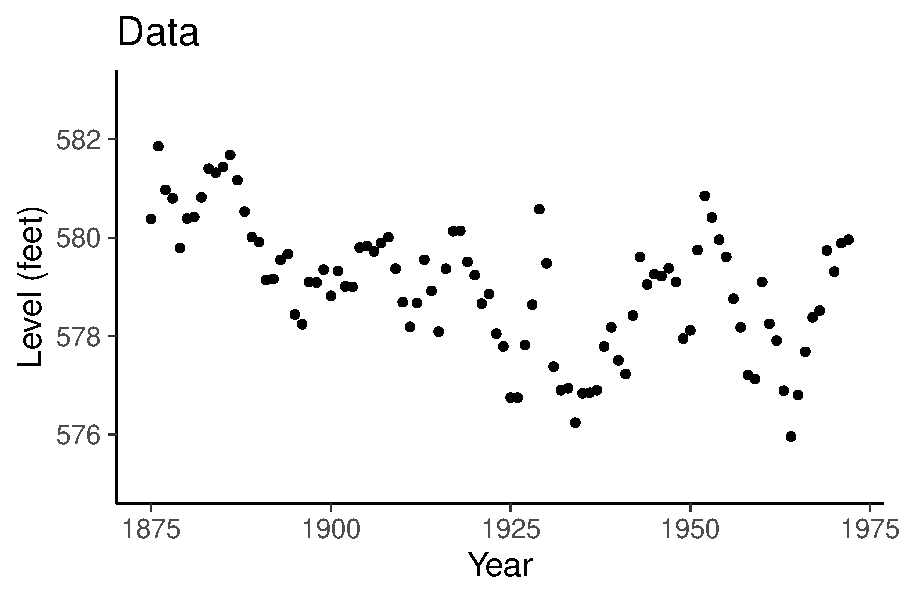
\includegraphics[width=8cm]{figs/lake4data.pdf}}
  \only<2>{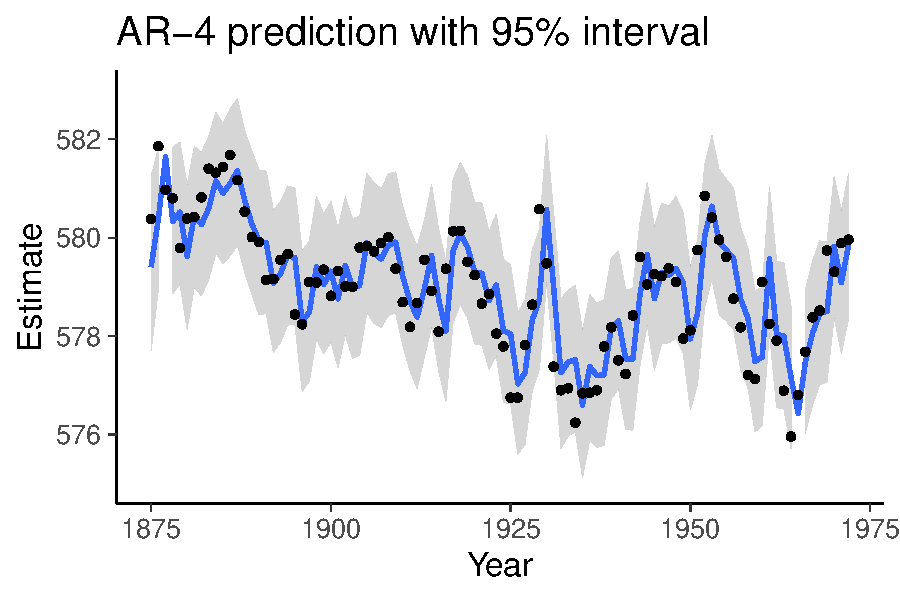
\includegraphics[width=8cm]{figs/lake4pred.pdf}}
  \only<3>{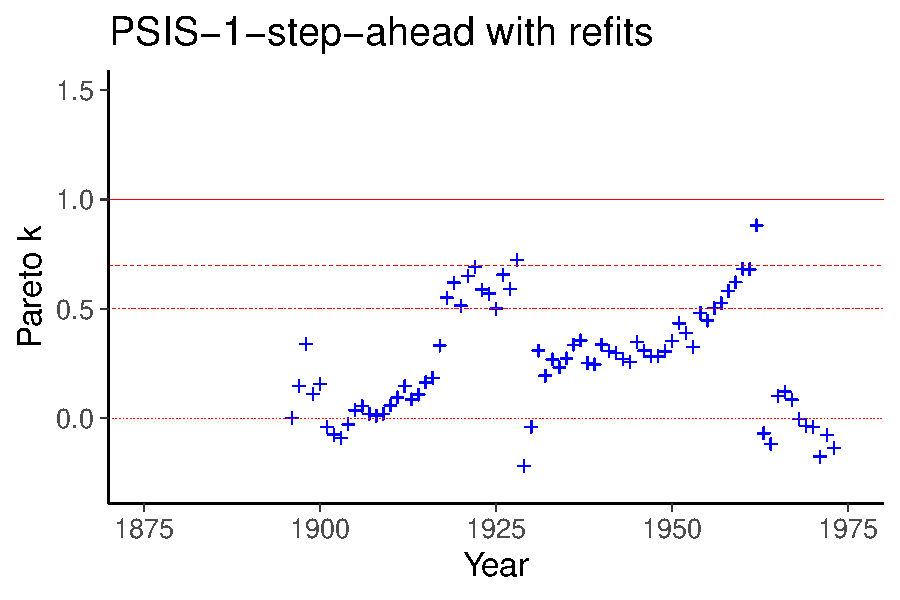
\includegraphics[width=8cm]{figs/lake4psisrefits.pdf}}

  \vspace{3\baselineskip}
  \only<3> {\small \url{mc-stan.org/loo/articles/loo2-lfo.html}}

\end{frame}


\subsection{K-fold CV}
\frame{\subsectionpage}

\begin{frame}{}

\frametitle{K-fold cross-validation}

\begin{itemize}
\item We can approximate $elpd_\text{loo}$ using K-fold CV
\pause
\begin{enumerate}
\item \texttt{for k in K}
  \begin{enumerate}
  \item hold $1/K$ observations out (i.e. $y_{-y(k)}$)
  \item compute $p(\theta|y_{-y(k)})$
  \item compute lpd for $y_{-y(k)}$
  \end{enumerate}
\item sum the lpd over $K$ folds
\end{enumerate}
\pause
\item We only need to estimate $K$ models
\end{itemize}

\end{frame}

\begin{frame}{}

\frametitle{K-fold cross-validation}

\begin{enumerate}
\item K-fold cross-validation can approximate LOO
  \begin{enumerate}
    \item can be used all uses for LOO
  \end{enumerate}
\item K-fold cross-validation can be used for hierarchical models
  \begin{enumerate}
    \item good for leave-one-group-out
  \end{enumerate}
\item K-fold cross-validation can be used for time series
  \begin{enumerate}
    \item with leave-block-out
  \end{enumerate}
\end{enumerate}

\end{frame}

\begin{frame}{}

  \only<1>{\includegraphics[width=8cm]{figs/lake3kfoldbal1.pdf}}
  \only<2>{\includegraphics[width=8cm]{figs/lake3kfoldbal2.pdf}}
  \only<3>{\includegraphics[width=8cm]{figs/lake3kfoldrand.pdf}}
  \only<4>{\includegraphics[width=8cm]{figs/rats1kfoldrand.pdf}}
  \only<5->{\includegraphics[width=8cm]{figs/rats1oneratb.pdf}}
  \\
%  \only<6>{kfold\_split\_random()\\ \vspace{0.2\baselineskip}
%  kfold\_split\_balanced()\\ \vspace{0.2\baselineskip}
%  kfold\_split\_stratified()}

\end{frame}

\begin{frame}{}

\frametitle{Cross-validation for model assessment}

\begin{enumerate}
\item CV is good for model assessment when application specific utility/cost functions are used
%  \begin{enumerate}
%  \item e.g. 90\% absolute error
%  \end{enumerate}
\item<2-> Also useful in model checking in similar way as posterior
  predictive checking (PPC)
  \begin{enumerate}
  \item model misspecification diagnostics\\ (e.g. Pareto-$k$ and p\_loo)
  \item checking calibration of leave-one-out predictive posteriors
    (ppc\_loo\_pit in bayesplot)
  \end{enumerate}
%  {\small see demos \url{avehtari.github.io/modelselection/}}
\end{enumerate}

\end{frame}

\subsection{Model Comparison}
\frame{\subsectionpage}


\begin{frame}{}
\frametitle{Model comparison}

 \begin{enumerate}
 \item ``A popular hypothesis has it that primates with larger brains
   produce more energetic milk, so that brains can grow quickly'' (from
   Statistical Rethinking)
   \begin{enumerate}
     \item Model 1: formula = kcal.per.g $\sim$ neocortex
     \item Model 2: formula = kcal.per.g $\sim$ neocortex + log(mass)
   \end{enumerate}
 \end{enumerate}

% \vspace{10\baselineskip}
% {\small \url{mc-stan.org/loo/articles/loo2-example.html}}

\end{frame}

\begin{frame}

   \only<1-2>{\includegraphics[width=8cm]{figs/milkelpdloo.pdf}}
   \only<3>{\includegraphics[width=8cm]{figs/milkelpdloo2.pdf}}
   \\
   \only<2-3>{Model 1 elpd\_loo $\approx$ 3.7, SE=1.8\\
   Model 2 elpd\_loo $\approx$ 8.4, SE=2.8}

\end{frame}

\begin{frame}[fragile]

   {\includegraphics[width=8cm]{figs/milkelpddiff.pdf}}
   \\
   {\scriptsize
 \begin{lstlisting}
 Model comparison:
 (negative 'elpd_diff' favors 1st model, positive favors 2nd)

 elpd_diff        se
       4.7       2.7
 \end{lstlisting}}

 \end{frame}

% \begin{frame}

% \frametitle{Arsenic well example -- Model comparison}


%    \includegraphics[width=.8\textwidth]{figs/arsenic12d.pdf}

%    An estimated difference in ${\rm elpd}_{\rm loo}$ of 16.4 with SE of 4.4.

% {\small see \href{http://link.springer.com/article/10.1007/s11222-016-9696-4}{Vehtari, Gelman \& Gabry (2017a)}}
%\end{frame}

\begin{frame}{}

\frametitle{Arsenic well example -- Model comparison}

\begin{enumerate}
\item Probability of switching well with high arsenic level in rural Bangladesh
  \begin{enumerate}
    \item Model 1 covariates: log(arsenic) and distance
    \item Model 2 covariates: log(arsenic), distance and education level
  \end{enumerate}
\end{enumerate}

\vspace{10\baselineskip}
{\small Gelman, Hill \& Vehtari (2020): Regression and Other Stories, Chapter 13.}

\end{frame}

\begin{frame}

\frametitle{Arsenic well example -- Model comparison}

  {\includegraphics[width=6.5cm]{figs/arsenicelpdloo.pdf}}
  % \only<3>{\includegraphics[width=8cm]{milkelpdloo2.pdf}}
  \\
  {Model 1 elpd\_loo $\approx$ -1952, SE=16\\
  Model 2 elpd\_loo $\approx$ -1938, SE=17}

\end{frame}



\begin{frame}[fragile]

\frametitle{Arsenic well example -- Model comparison}

  {\includegraphics[width=6.5cm]{figs/arsenicelpddiff.pdf}}
  \\
  {\scriptsize
\begin{lstlisting}
> loo_compare(model1, model2)
       elpd_diff se_diff
model2   0.0       0.0
model1 -14.4       6.1
\end{lstlisting}}
\vspace{-\baselineskip}
    {\scriptsize \hspace{6cm} see \href{http://link.springer.com/article/10.1007/s11222-016-9696-4}{Vehtari, Gelman \& Gabry (2017a)}}

\end{frame}

\begin{frame}[fragile]

\frametitle{Arsenic well example -- Model comparison}

  {\scriptsize
\begin{lstlisting}
> loo_compare(model1, model2)
       elpd_diff se_diff
model2   0.0       0.0
model1 -14.4       6.1
\end{lstlisting}}

    {\tt se\_diff} and normal approximation for the uncertainty in the
    difference is good only if models are well specified and the
    number of observations is relatively big.

%\vspace{9\baselineskip}
%    {\scriptsize \hspace{6cm} see \href{http://link.springer.com/article/10.1007/s11222-016-9696-4}{Vehtari, Gelman \& Gabry (2017a)}}

\end{frame}



\begin{frame}{}

\frametitle{What if one is not clearly better than others?}

  \begin{enumerate}
  \item<2-> Continuous expansion including all models?
    \begin{enumerate}
    \item and then analyse the posterior distribution directly
  %      {\small \url{avehtari.github.io/modelselection/betablockers.html}}
      \item sparse priors like regularized horseshoe prior instead of variable selection
  %      {\small video, refs and demos at
    %      \url{avehtari.github.io/modelselection/}}
    \end{enumerate}
  \item<3-> Model averaging with BMA or Bayesian stacking?
    %{\small \url{mc-stan.org/loo/articles/loo2-example.html}}
  \item<4-> In a nested case choose simpler if assuming some cost for
    extra parts?
%    {\small \url{andrewgelman.com/2018/07/26/parsimonious-principle-vs-integration-uncertainties/}}
  \item<5-> In a nested case choose more complex if you want to take
    into account all the uncertainties.%\\
%    {\small \url{andrewgelman.com/2018/07/26/parsimonious-principle-vs-integration-uncertainties/}}
  \end{enumerate}

\end{frame}


\begin{frame}{}

\frametitle{Cross-validation and model selection}

  \begin{enumerate}
  \item<1-> Cross-validation can be used for model selection if
    \begin{enumerate}
      \item small number of models
      \item the difference between models is clear
    \end{enumerate}
  \item<2-> Do not use cross-validation to choose from a large set of models
    \begin{enumerate}
    \item selection process leads to overfitting
    % \item you may use projection predictive approach
    % \item useful when correlating variables make the posterior
    %   distribution analysis difficult\\
    %   {\small video, refs and demos  at \url{avehtari.github.io/modelselection/}\\
    %   and \href{http://link.springer.com/article/10.1007/s11222-016-9649-y}{Piironen \& Vehtari (2017)}}
    \end{enumerate}
  \item<3-> Overfitting in selection process is not unique for cross-validation
  \end{enumerate}
\end{frame}

\begin{frame}



\frametitle{Selection induced bias and overfitting}

  \begin{itemize}
  \item Selection induced bias in cross-validation
    \begin{itemize}
    \item same data is used to assess the performance and make the selection
    \item the selected model fits more to the data
    \item the CV estimate for the selected model is biased
%    \item recognized already, e.g., by Stone (1974)
    \end{itemize}
    \pause
  \item Performance of the selection process itself can be assessed
    using two level cross-validation, but it does not help choosing
    better models
    \pause
  \item Bigger problem if there is a large number of models as in
    covariate selection
  \end{itemize}

\end{frame}

%\begin{frame}

%\frametitle{Selection induced bias in variable selection}

%  \includegraphics[width=\textwidth]{figs/cv.pdf}

%\end{frame}

%\begin{frame}

%\frametitle{Selection induced bias in variable selection}

%  \includegraphics[height=0.88\textheight]{figs/simulated_searchpath.pdf}
%   \vspace{-1.5\baselineskip}
%   \mbox{{\hspace{8cm} \footnotesize \href{http://link.springer.com/article/10.1007/s11222-016-9649-y}{Piironen \& Vehtari (2017)}}}

%\end{frame}



\section{Information criteria}
\frame{\sectionpage}

% The problem with parameters in bayeisan stats

% AIC and DIC with math
% Limit p(y|\theta) with theta

% WAIC

\begin{frame}{}

\frametitle{ WAIC vs PSIS-LOO}

\begin{enumerate}
  \item<2-> WAIC has same assumptions as LOO
  \item<3-> PSIS-LOO is more accurate
  \item<4-> PSIS-LOO has much better diagnostics
  \item<5-> LOO makes the prediction assumption more clear,\\ which
    helps if K-fold-CV is needed instead
  \item<6-> Multiplying by -2 doesn't give any benefit\\ (Watanabe
    didn't multiply by -2)
\end{enumerate}

\vspace{6\baselineskip}
{\small see \href{http://link.springer.com/article/10.1007/s11222-016-9696-4}{Vehtari, Gelman \& Gabry (2017a)}}
\end{frame}

\begin{frame}{}

\frametitle{ *IC}

\begin{enumerate}
  \item AIC uses maximum likelihood estimate for prediction
  \item DIC uses posterior mean for prediction
  \item BIC is an approximation for marginal likelihood
  \item TIC, NIC, RIC, PIC, BPIC, QIC, AICc, ...
\end{enumerate}

\end{frame}


\section{Model averaging}
\frame{\sectionpage}


%\begin{frame}{}

%\frametitle{ Marginal likelihood / Bayes factor}

%\vspace{-0.3\baselineskip}
%\begin{enumerate}
%\item Like leave-future-out 1-step-ahead cross-validation but starting with 0 observations\\
%  \onslide<3->{- which makes it very sensitive to prior}
%  \onslide<4->{and \\- unstable in case of misspecified
%    models}\uncover<5->{ also asymptotically}
%\end{enumerate}
%\vspace{-0.5\baselineskip}
%  \onslide<2->{\includegraphics[width=9.4cm]{figs/lake3bf.pdf}}

%\end{frame}


%\begin{frame}

%\frametitle{Model averaging}

%  \begin{enumerate}
%  \item<+-> Prefer continuous model expansion
%  \item<+-> If needed integrate over the model space = model averaging
%  \item<+-> Bayesian stacking may work better than BMA
%    \begin{enumerate}
%    \item \href{https://projecteuclid.org/euclid.ba/1516093227}{Yao, Vehtari, Simpson, \& Gelman (2018)}
%    \end{enumerate}
%  \end{enumerate}

%\end{frame}




\section{Summary}
\frame{\sectionpage}

\begin{frame}{}

\frametitle{Take-home messages}

  \begin{enumerate}
  \item It's good to think predictions of observables, because
    observables are the only ones we can observe
  \item \only<1>{\color{gray}}Cross-validation can simulate predicting and observing new
    data
  \item \only<2>{\color{gray}}Cross-validation is good if you don't
    trust your model
  \item \only<3>{\color{gray}}Different variants of cross-validation
    are useful in different scenarios
  \item \only<4>{\color{gray}}Cross-validation has high variance, and
    {\bf if} you trust your model you can beat cross-validation in
    accuracy
  \end{enumerate}
  \only<5>{~}

\end{frame}

%\subsection{Additional reading}
%\frame{\sectionpage}


%%%%%%%%%%%%%%%%%%%%%%%%%%%%%%%%%%%%%%%%%%%%%%%%%%%%%%%%%%%%%%%%%%


\end{document}
